%% BioMed_Central_Tex_Template_v1.06
%%                                      %
%  bmc_article.tex            ver: 1.06 %
%                                       %

%%IMPORTANT: do not delete the first line of this template
%%It must be present to enable the BMC Submission system to
%%recognise this template!!

%%%%%%%%%%%%%%%%%%%%%%%%%%%%%%%%%%%%%%%%%
%%                                     %%
%%  LaTeX template for BioMed Central  %%
%%     journal article submissions     %%
%%                                     %%
%%          <8 June 2012>              %%
%%                                     %%
%%                                     %%
%%%%%%%%%%%%%%%%%%%%%%%%%%%%%%%%%%%%%%%%%

%%%%%%%%%%%%%%%%%%%%%%%%%%%%%%%%%%%%%%%%%%%%%%%%%%%%%%%%%%%%%%%%%%%%%
%%                                                                 %%
%% For instructions on how to fill out this Tex template           %%
%% document please refer to Readme.html and the instructions for   %%
%% authors page on the biomed central website                      %%
%% https://www.biomedcentral.com/getpublished                      %%
%%                                                                 %%
%% Please do not use \input{...} to include other tex files.       %%
%% Submit your LaTeX manuscript as one .tex document.              %%
%%                                                                 %%
%% All additional figures and files should be attached             %%
%% separately and not embedded in the \TeX\ document itself.       %%
%%                                                                 %%
%% BioMed Central currently use the MikTex distribution of         %%
%% TeX for Windows) of TeX and LaTeX.  This is available from      %%
%% https://miktex.org/                                             %%
%%                                                                 %%
%%%%%%%%%%%%%%%%%%%%%%%%%%%%%%%%%%%%%%%%%%%%%%%%%%%%%%%%%%%%%%%%%%%%%

%%% additional documentclass options:
%  [doublespacing]
%  [linenumbers]   - put the line numbers on margins

%%% loading packages, author definitions

\documentclass[twocolumn]{bmcart}% uncomment this for twocolumn layout and comment line below
%\documentclass{bmcart}

%%% Load packages
\usepackage{amsthm,amsmath}
\usepackage{nccmath}
%\RequirePackage[numbers]{natbib}
%\RequirePackage[authoryear]{natbib}% uncomment this for author-year bibliography
\RequirePackage{hyperref}
\usepackage{multirow}
\usepackage[utf8]{inputenc} %unicode support
%\usepackage[applemac]{inputenc} %applemac support if unicode package fails
%\usepackage[latin1]{inputenc} %UNIX support if unicode package fails
\usepackage{booktabs}% http://ctan.org/pkg/booktabs
\urlstyle{same} % URL fonts are not wide mono
\usepackage{graphicx} %render plots.. 
\usepackage{lipsum}
\usepackage{cite}
\renewcommand*{\citedash}{\hbox{-}\penalty\citepunctpenalty}
%%%%%%%%%%%%%%%%%%%%%%%%%%%%%%%%%%%%%%%%%%%%%%%%%
%%                                             %%
%%  If you wish to display your graphics for   %%
%%  your own use using includegraphic or       %%
%%  includegraphics, then comment out the      %%
%%  following two lines of code.               %%
%%  NB: These line *must* be included when     %%
%%  submitting to BMC.                         %%
%%  All figure files must be submitted as      %%
%%  separate graphics through the BMC          %%
%%  submission process, not included in the    %%
%%  submitted article.                         %%
%%                                             %%
%%%%%%%%%%%%%%%%%%%%%%%%%%%%%%%%%%%%%%%%%%%%%%%%%

%\def\includegraphic{}
%\def\includegraphics{}

%%% Put your definitions there:
\startlocaldefs
\endlocaldefs

%%% Begin ...
\begin{document}

%%% Start of article front matter
\begin{frontmatter}

\begin{fmbox}
\dochead{Research}

%%%%%%%%%%%%%%%%%%%%%%%%%%%%%%%%%%%%%%%%%%%%%%
%%                                          %%
%% Enter the title of your article here     %%
%%                                          %%
%%%%%%%%%%%%%%%%%%%%%%%%%%%%%%%%%%%%%%%%%%%%%%

\title{Developing a prognostic model for biochemical recurrence in prostate cancer using a novel circRNA-miRNA-mRNA regulatory network}

%%%%%%%%%%%%%%%%%%%%%%%%%%%%%%%%%%%%%%%%%%%%%%
%%                                          %%
%% Enter the authors here                   %%
%%                                          %%
%% Specify information, if available,       %%
%% in the form:                             %%
%%   <key>={<id1>,<id2>}                    %%
%%   <key>=                                 %%
%% Comment or delete the keys which are     %%
%% not used. Repeat \author command as much %%
%% as required.                             %%
%%                                          %%
%%%%%%%%%%%%%%%%%%%%%%%%%%%%%%%%%%%%%%%%%%%%%%

\author[
  addressref={aff1},                   % id's of addresses, e.g. 
    %corref={aff1}, %% NOTE TO EDITOR: I had to comment this line to avoid bmc@corref@authorthanks undefined errors - very confusing.. 
    email={b.digby1@universityofgalway.ie}  % email address
]{\inits{B.D.}\fnm{Barry} \snm{Digby}}
\author[
  addressref={aff2},
  email={Stephen.Finn@tcd.ie}
]{\inits{S.P.F}\fnm{Stephen P.} \snm{Finn}}
\author[
  addressref={aff1},
  email={pilib.obroin@universityofgalway.ie}
]{\inits{P.O.B.}\fnm{Pilib} \snm{\'O Broin}}


%%%%%%%%%%%%%%%%%%%%%%%%%%%%%%%%%%%%%%%%%%%%%%
%%                                          %%
%% Enter the authors' addresses here        %%
%%                                          %%
%% Repeat \address commands as much as      %%
%% required.                                %%
%%                                          %%
%%%%%%%%%%%%%%%%%%%%%%%%%%%%%%%%%%%%%%%%%%%%%%

\address[id=aff1]{%                           % unique id
  \orgdiv{School of Mathematical and Statistical Sciences},             % department, if any
  \orgname{University of Galway},          % university, etc
  \city{Galway},                              % city
  \cny{Ireland}                                    % country
}
\address[id=aff2]{%
  \orgdiv{Department of Histopathology and Morbid Anatomy},
  \orgname{Trinity Translational Medicine Institute},
  %\street{},
  %\postcode{}
  \city{Dublin},
  \cny{Ireland}
}

%%%%%%%%%%%%%%%%%%%%%%%%%%%%%%%%%%%%%%%%%%%%%%
%%                                          %%
%% Enter short notes here                   %%
%%                                          %%
%% Short notes will be after addresses      %%
%% on first page.                           %%
%%                                          %%
%%%%%%%%%%%%%%%%%%%%%%%%%%%%%%%%%%%%%%%%%%%%%%

%\begin{artnotes}
%%\note{Sample of title note}     % note to the article
%\note[id=n1]{Equal contributor} % note, connected to author
%\end{artnotes}

%\end{fmbox}% comment this for two column layout

%%%%%%%%%%%%%%%%%%%%%%%%%%%%%%%%%%%%%%%%%%%%%%%
%%                                           %%
%% The Abstract begins here                  %%
%%                                           %%
%% Please refer to the Instructions for      %%
%% authors on https://www.biomedcentral.com/ %%
%% and include the section headings          %%
%% accordingly for your article type.        %%
%%                                           %%
%%%%%%%%%%%%%%%%%%%%%%%%%%%%%%%%%%%%%%%%%%%%%%%

\begin{abstractbox}
% 205 words - max is 350
\begin{abstract}
\parttitle{Background} 
Biochemical recurrence (BCR) occurs in one-third of prostate cancer patients treated with local therapy and inevitably develops in all patients treated with enzalutamide. In this study, we combined both PCa and enzalutamide-resistance signatures to derive a model for effective prediction of BCR in prostate cancer.

\parttitle{Methods} 
Differentially expressed circRNAs, miRNAs and mRNAs were incorporated from multiple studies to derive a competing endogenous RNA (ceRNA) regulatory network. A prognostic model was constructed from the network using Cox regression and stepwise regression. The model was further tested on six external validation datasets to evaluate the efficacy of the prognostic model in predicting BCR. Pathway analysis and immune infiltration analysis was computed on a per-sample basis to identify differences in high-risk and low-risk patients.    

\parttitle{Results}
The linear predictors from the 4-gene prognostic model effectively stratified patients into high-risk and low-risk strata with significantly different BCR outcomes. High-risk patients exhibited unfavourable prognosis and elevated immune infiltration compared to low-risk groups. Moreover, the prognostic model exhibited high prediction accuracy in classifying patients with BCR events in both the derivation and validation datasets. 

\parttitle{Conclusion}
We present a first-of-kind circRNA-miRNA-mRNA regulatory network derived from prostate cancer and enzalutamide-resistant cells. The prognostic ceRNA network offers insights into the potential regulatory mechanism of non-coding RNAs in BCR.


\end{abstract}

%%%%%%%%%%%%%%%%%%%%%%%%%%%%%%%%%%%%%%%%%%%%%%
%%                                          %%
%% The keywords begin here                  %%
%%                                          %%
%% Put each keyword in separate \kwd{}.     %%
%%                                          %%
%%%%%%%%%%%%%%%%%%%%%%%%%%%%%%%%%%%%%%%%%%%%%%

\begin{keyword}
\kwd{Prostate cancer}
\kwd{Enzalutamide}
\kwd{Biochemical recurrence}
\kwd{Prognostic signature}
\kwd{Competing endogenous RNA network}
\end{keyword}

% MSC classifications codes, if any
%\begin{keyword}[class=AMS]
%\kwd[Primary ]{}
%\kwd{}
%\kwd[; secondary ]{}
%\end{keyword}

\end{abstractbox}
%
\end{fmbox}% uncomment this for two column layout

\end{frontmatter}

%%%%%%%%%%%%%%%%%%%%%%%%%%%%%%%%%%%%%%%%%%%%%%%%
%%                                            %%
%% The Main Body begins here                  %%
%%                                            %%
%% Please refer to the instructions for       %%
%% authors on:                                %%
%% https://www.biomedcentral.com/getpublished %%
%% and include the section headings           %%
%% accordingly for your article type.         %%
%%                                            %%
%% See the Results and Discussion section     %%
%% for details on how to create sub-sections  %%
%%                                            %%
%% use \cite{...} to cite references          %%
%%  \cite{koon} and                           %%
%%  \cite{oreg,khar,zvai,xjon,schn,pond}      %%
%%                                            %%
%%%%%%%%%%%%%%%%%%%%%%%%%%%%%%%%%%%%%%%%%%%%%%%%

%%%%%%%%%%%%%%%%%%%%%%%%% start of article main body
% <put your article body there>

%%%%%%%%%%%%%%%%
%% Background %%
%%
\section*{Background}
Prostate cancer (PCa) is the second most frequent cancer and the fifth leading cause of cancer-associated deaths in men \cite{Sung2021May}. Radical prostatectomy, external beam radiotherapy or brachytherapy are the mainstay of treatment for localized PCa. Approximately 35\% of men experience biochemical recurrence (BCR) after treatment as defined by three consecutive rises in prostate-specific antigen (PSA) levels 1 week apart, progressing to castrate-resistant PCa (CRPC) \cite{Lim2018Aug}. Treatment courses for CRPC involve the abrogation of androgen receptor (AR) signalling, preventing its translocation to the nucleus and binding to DNA \cite{Cornford2017Apr}. Enzalutamide is one such second-generation anti-androgen drug that competitively binds the ligand binding domain of the AR impeding AR signalling. Despite overall survival benefits of 4.8 months in patients, between 20\% - 40\% are intrinsically resistant whilst all will eventually acquire resistance to the drug as measured by increasing PSA levels \cite{Scher2012Sep, Lim2018Aug} indicative of BCR. There is therefore an increasing need to identify biomarkers associated with BCR in CRPC and enzalutamide-resistant patients. \par

\begin{table*}[hbt!]
\caption{Prostate cancer datasets used in the study.}
\begin{tabular}{lllll}
\toprule 
\textbf{Data type} & \textbf{Series} & \textbf{Platform} & \textbf{Sample size tumor} & \textbf{Sample size normal} 
\\
\toprule 
circRNA & \href{https://www.ncbi.nlm.nih.gov/geo/query/acc.cgi?acc=GSE113153}{GSE113153} \cite{Yang2019Apr} & GPL21825 & 10 & 0
\\
miRNA & \href{https://www.ncbi.nlm.nih.gov/geo/query/acc.cgi?acc=GSE21036}{GSE21036} \cite{Taylor2010Jul} & GPL8227 & 100 & 28 
\\ 
miRNA & \href{https://www.ncbi.nlm.nih.gov/geo/query/acc.cgi?acc=GSE23022}{GSE23022} \cite{Wach2012Feb} & GPL8786 & 20 & 20 
\\
miRNA & \href{https://www.ncbi.nlm.nih.gov/geo/query/acc.cgi?acc=GSE36803}{GSE36803} \cite{Lin2013Feb} & GPL8786 & 21 & 21 
\\ 
miRNA & \href{https://www.ncbi.nlm.nih.gov/geo/query/acc.cgi?acc=GSE45604}{GSE45604} \cite{Casanova-Salas2014Jul} & GPL14613 & 50 & 10 
\\ 
miRNA & \href{https://www.ncbi.nlm.nih.gov/geo/query/acc.cgi?acc=GSE46738}{GSE46738} \cite{Leite2015Jan} & GPL8786 & 53 & 4 
\\ 
miRNA & \href{https://portal.gdc.cancer.gov/repository}{TCGA} \cite{Grossman2016Sep} & PRAD & 498 & 52 
\\
mRNA & \href{https://portal.gdc.cancer.gov/repository}{TCGA} \cite{Grossman2016Sep} & PRAD & 498 & 52
\\
\toprule
\end{tabular}
\label{tab:pca_datasets}
\end{table*}

\begin{table*}[hbt!]
\caption{Enzalutamide datasets used in the study.}
\begin{tabular}{lllll}
\toprule
\textbf{Data type} & \textbf{Series} & \textbf{Platform} & \textbf{Description of LNCaP samples} 
\\
\toprule
circRNA & \href{https://www.ncbi.nlm.nih.gov/geo/query/acc.cgi?acc=GSE118959}{GSE118959} \cite{Greene2019Jul,Lim2021Dec} & GPL21825 & Clone 1, Clone 9, Control (n=3)
\\
miRNA & \textit{in-house} & Illumina TruSeq & Clone 1, Clone 9, Control (n=3)
\\
mRNA & \href{https://www.ncbi.nlm.nih.gov/geo/query/acc.cgi?acc=GSE143408}{GSE143408} \cite{KaylynD.Tousignant2020Jun} & GPL25684 & 21, 14, 7, 0 days Enz trt (n=3)
\\
mRNA & \href{https://www.ncbi.nlm.nih.gov/geo/query/acc.cgi?acc=GSE78201}{GSE78201} \cite{Kregel2016May} & GPL10558 & 6 months Enz trt, control (n=4)
\\
mRNA & \href{https://www.ncbi.nlm.nih.gov/geo/query/acc.cgi?acc=GSE88752}{GSE88752} \cite{Li2018Sep} & GPL11154 & Enz trt, Enz sensitive (n=4)
\\
mRNA & \textit{in-house} & Illumina NovaSeq & Clone 1, Clone 9, Control (n=3)
\\
\toprule
\end{tabular}
\label{tab:enz_datasets}
\end{table*}

Next generation sequencing (NGS) provides researchers with a powerful tool to detect biomarkers in clinical samples. The preparation times, sequencing time and costs associated with NGS technologies are constantly dropping, making NGS a cost-effective tool for biomarker discovery \cite{Lopez2015Dec}. RNA biomarkers are of particular interest, providing a snapshot of the dynamic cellular states compared to DNA biomarkers and exhibit superior sensitivity and specificity compared to protein biomarkers \cite{Nimse2016,Xi2017Mar}. Taken together, RNA biomarkers not only provide clinical utility but can also refine our knowledge of underlying disease aetiology. \par

The ENCODE project revealed 76\% of the human genome is transcribed, but only 1.2\% of this represents protein-coding genes \cite{BibEntry2012Sep, Djebali2012Sep} resulting in an increased interest in non-coding RNAs (ncRNAs) and their role in gene regulation. ncRNAs can be categorised as small ncRNAs ($<$200nt length) comprising micro RNAs (miRNAs), piwi-interacting RNAs (piRNAs), small nucleolar RNAs (snoRNAs) and long non-coding RNAs (lncRNAs) ($>$ 200nt length). More recently, circular RNAs (circRNAs), originally believed to be aberrant by-products of splicing \cite{Cocquerelle1993Jan, Qian1992}, have emerged as a class of ncRNAs. circRNAs harbour functionally active and evolutionarily conserved miRNA response elements (MRE) within their mature spliced sequence capable of sequestering miRNAs and have been proposed to act as competitive endogenous RNAs (ceRNAs) in circRNA-miRNA-mRNA regulatory networks \cite{Thomas2014, Hansen2013, DENZLER2014}. Several studies detailing the role of ncRNAs in PCa have since emerged, identifying potential molecular biomarkers, new therapeutic strategies and advancing our understanding of disease progression \cite{Aird2018Mar, longandshort, Ghiam2017Apr, Ding2021Jun, Takayama}.  \par

The tumor microenvironment (TME) represents a complex ecosystem of neoplastic cells, extracellular matrix (ECM), and nonneoplastic cells, including resident mesenchymal support cells, endothelial cells, and infiltrated inflammatory immune cells. Whether by cause or consequence, aberrant innate and adaptive immune responses contribute to the tumorigenesis of early stage cancers by applying selective pressure to tumor cells, preferentially selecting aggressive clones, inducing immunosuppression and stimulating tumor cell proliferation \cite{Gonzalez2018Oct}. In clinically detectable cancers, T cell infiltration has been reported to improve patient outcomes \cite{Dieu-Nosjean2008Sep}. Conversely, macrophage populations (M2-like polarisation) are associated with worse outcome \cite{Mantovani2017Jul}. It is therefore of interest to characterise the immune cell subpopulations to identify putative markers for disease progression. Whilst progress has been made on this front in studies of the PCa TME, results are largely conflicting owing to the heterogeneous nature of PCa \cite{Apusiga2023Dec}.  

In this study, we combine multiple circRNA, miRNA, mRNA PCa and enzalutamide-resistant expression datasets to derive a competing endogenous RNA (ceRNA) network. Using the mRNAs in the network, we derived a prognostic signature for the prediction of BCR in patients using The Cancer Genome Atlas Prostate Adenocarcinoma (TCGA-PRAD) dataset. The effectiveness of the prognostic signature was demonstrated using TCGA-PRAD and six external PCa datasets, where patients were stratified into high-risk and low-risk categories showing distinctly different BCR outcomes. By combining the prognostic index obtained from the 4-gene prognostic signature with clinical features, we derived a clinical nomogram for clinical use. Furthermore, we detail the TME in high-risk and low-risk stratum via immune infiltration analysis to add to the growing knowledge base of immune-cell based biomarkers in PCa.  



\section*{Methods}
\subsection*{\textbf{Data collection}}
The Gene Expression Omnibus (GEO) \cite{Edgar2002Jan} (\url{https://www.ncbi.nlm.nih.gov/geo/}) was used to access publicly available microarray and RNA-Sequencing datasets that contain circRNA, miRNA and mRNA expression profiles of prostate cancer patients and LNCaP cell lines treated with enzalutamide. circRNA microarray datasets were screened using the search term ("GPL21825[Accession] AND ("prostatic neoplasms"[MeSH Terms] OR prostate cancer[All Fields]) AND ("g se"[Filter] AND "Non-coding RNA profiling by array"[Filter])"). miRNA datasets were screened using the search term ("prostate"[MeSH Terms] OR prostate[All Fields]) AND ("micrornas"[All Fields] OR "micrornas"[MeSH Terms] OR miRNA[All Fields]) AND LNCaP[All Fields]"). Finally, mRNA datasets were screened using the search term ("enzalutamide" [All Fields] OR ("enzalutamide"[All Fields] OR enzalutamide[All Fields]) AND "LNCaP"[All Fields] AND "gse"[Filter]).\par
In addition to the selected GEO datasets, TCGA-PRAD miRNA and mRNA expression datasets were downloaded from the GDC portal \cite{Grossman2016Sep} (\url{https:// portal.gdc.cancer.gov/)} on July 25\textsuperscript{th} 2023. In-house sequencing of enzalutamide-resistant LNCaP cell lines was performed to generate miRNA and mRNA expression data to supplement the construction of the circRNA-miRNA-mRNA network. Descriptions of samples used in each dataset for differential expression analysis and network construction are provided (Table \ref{tab:pca_datasets}, Table \ref{tab:enz_datasets}). \par
With respect to modelling a prognostic signature, the TCGA-PRAD mRNA dataset was used as the derivation dataset. The Belfast (\href{https://www.ncbi.nlm.nih.gov/geo/query/acc.cgi?acc=GSE116918}{GSE116918} \cite{Belfast}), CPC (\href{https://www.ncbi.nlm.nih.gov/geo/query/acc.cgi?acc=GSE107299}{GSE107299} \cite{CPC}), DKFZ (\href{https://ega-archive.org/studies/EGAS00001002923}{EGAS00001002923} \cite{DKFZ}), Long et al. 2014 (\href{https://www.ncbi.nlm.nih.gov/geo/query/acc.cgi?acc=GSE54460}{GSE54460} \cite{GSE54460}), Taylor et al. 2010 (\href{https://www.ncbi.nlm.nih.gov/geo/query/acc.cgi?acc=GSE21034}{GSE21034} \cite{Taylor}), Ross-Adams et al. 2014 (Stockholm, \href{https://www.ncbi.nlm.nih.gov/geo/query/acc.cgi?acc=GSE70769}{GSE70769} \cite{Stockholm}) PCa datasets were used as validation datasets for the prognostic model.


\subsection*{\textbf{Data processing and differential expression analysis of circRNAs, miRNAs and mRNAs}}
GSE113153, GSE118959, GSE45604, GSE46738, GSE-143408 and GSE78201 quantile normalized log2 transformed circRNA, miRNA and mRNA microarray datasets were downloaded using GEOquery \cite{Davis2007Jul} and analysed in R (version 4.2.0). GSE21036, GSE23022 and GSE36803 miRNA and mRNA raw CEL files were downloaded from ArrayExpress \cite{Parkinson2007Jan} (\url{http://www.ebi.ac.uk/arrayexpress}), requiring log2 RMA normalization using the oligo package \cite{Carvalho2010Oct} prior to differential expression analysis. GSE88752, TCGA-PRAD miRNA and TCGA-PRAD mRNA count data were normalized with respect to library size using edgeR \cite{Robinson2010Jan} and transformed using limma-voom \cite{Law2014Feb}. In-house LNCaP small RNA-Sequencing data was processed in the following manner: 1) download, process and generate indices using the miRBase hairpin FASTA file \cite{Bowtie, Shen2016Oct}; 2) removal of adapter sequences and read filtering \cite{Krueger2023Feb}; 3) collapse filtered reads \cite{Pantano2016Mar}; 4) align collapsed reads to the hairpin \cite{Bowtie}; 5) quantify miRNAs using miRBase GFF file \cite{Desvignes2020Feb}. The in-house LNCaP RNA-Sequencing samples were processed using the `STAR-Salmon' transcript quantification subworkflow in nf-core/rnaseq \cite{Patel2023Jun}.
\par
Limma \cite{Ritchie2015Apr} was used to identify differentially expressed circRNAs/miRNAs/mRNAs between contrasts of interest; genes with an adjusted p-value $\leq$ 0.05 after Benjamini-Hochberg multiple testing correction were deemed statistically significant. Candidate circRNA/miRNA/mRNAs identified by differential expression analysis for network construction were screened by the following criteria: 1) circRNAs must be present in GSE118959 Clone 1 vs. control (high enzalutamide resistance) and one of GSE118959 Clone 9 vs. control (moderate enzalutamide resistance) or GSE113153 Gleason high $\geq$8 vs. Gleason low $<$8; 2) miRNAs must be present in LNCaP Clone 1 vs. control (high enzalutamide resistance) and at least one of GSE21036, GSE23022, GSE36803, GSE46738, GSE46738 or TCGA-PRAD (tumor vs. normal); 3) mRNAs must be present in LNCaP Clone 1 vs. control (high enzalutamide resistance), TCGA-PRAD (tumor vs. normal) and one of GSE88752, GSE143408, GSE78201 enzalutamide-resistant datasets. 4) common circRNAs/miRNAs/mRNAs identified must exhibit the same fold-change direction in the limma topTable results from which they originate. Customised scripts were used to convert both Arraystar human circRNA microarray V2 probes to circbase IDs and outdated miRNA probe IDs to the latest miRBase alias to ensure standardization of results and compatibility with downstream target prediction analysis. 

\subsection*{\textbf{circRNA, miRNA, mRNA target prediction }}
 
The predicted targets of screened differentially expressed (DE) circRNAs were obtained using the CircBase database \cite{Glazar2014Nov} (\url{http://www.circbase.org/}) and the Cancer-Specific CircRNA Database \cite{Xia2018Jan} (\url{http://gb.whu.edu.cn/CSCD/}), generating database-guided circRNA-miRNA pairs. Candidate DE-miRNAs for the ceRNA network were subset via the intersection of the predicted circRNA-miRNA targets. Finally, the gene targets of DE-miRNAs were obtained using miRBase \cite{Kozomara2019Jan} (\url{https://www.mirbase.org/}), miRTarBase \cite{Hsu2011Jan} (\url{https://mirtarbase.cuhk.edu.cn/}), miRNet \cite{Chang2020Jul} (\url{https://www.mirnet.ca/miRNet/home.xhtml} (a user-submitted list of miRNAs)) and TargetScan \cite{Targetscan} (\url{https://www.targetscan.org/vert_80/}) and overlapped with DE-mRNAs for ceRNA network construction.

\begin{table*}[ht!]
\caption{Differentially expressed RNAs returned by Limma.}
\begin{tabular}{lllll}
\toprule 
\textbf{Data type} & \textbf{Series} & \textbf{Contrast} & \textbf{Up-regulated} & \textbf{Down-regulated} 
\\
\toprule 
circRNA & GSE113153 & Gleason high vs. low & 2761 & 2245
\\
circRNA & GSE118959 & Clone 1 vs. control & 649 & 771 
\\ 
circRNA & GSE118959 & Clone 9 vs. control & 20 & 79 
\\ 
\toprule
& & Unique overlapping circRNAs: & 174 & 105
\\
\toprule
miRNA & GSE21036 & Tumor vs. normal & 153 & 146
\\ 
miRNA & GSE23022 & Tumor vs. normal & 17 & 8 
\\ 
miRNA & GSE36803 & Tumor vs. normal & 36 & 92
\\ 
miRNA & GSE45604 & Tumor vs. normal & 22 & 67 
\\
miRNA & GSE46738 & Tumor vs. normal & 68 & 68
\\
miRNA & LNCaP & Clone 1 vs. control & 146 & 110 
\\ 
miRNA & LNCaP & Clone 9 vs. control & 4 & 1
\\
miRNA & TCGA-PRAD & Tumor vs. normal & 130 & 128
\\
\toprule
& & Unique overlapping miRNAs: & 16 & 26
\\
\toprule 
mRNA & GSE143408 & 7 days vs. 0 days & 3829 & 3458
\\
mRNA & GSE143408 & 14 days vs. 0 days & 5693 & 4792
\\
mRNA & GSE143408 & 21 days vs. 0 days & 6128 & 4977
\\
mRNA & GSE78201 & 6 months vs. control & 518 & 571
\\
mRNA & GSE88752 & ADT + ENZ vs. control & 3564 & 2942
\\
mRNA & LNCaP & Clone 1 vs. control & 4686 & 4379 
\\
mRNA & LNCaP & Clone 9 vs. control & 1420 & 1303
\\
mRNA & TCGA-PRAD & Tumor vs. normal & 3860 & 4506 
\\
\toprule
& & Unique overlapping mRNAs: & 196 & 172 
\\
\toprule
\end{tabular}
\label{tab:de_results}
\end{table*}

\begin{figure*}[ht!]
    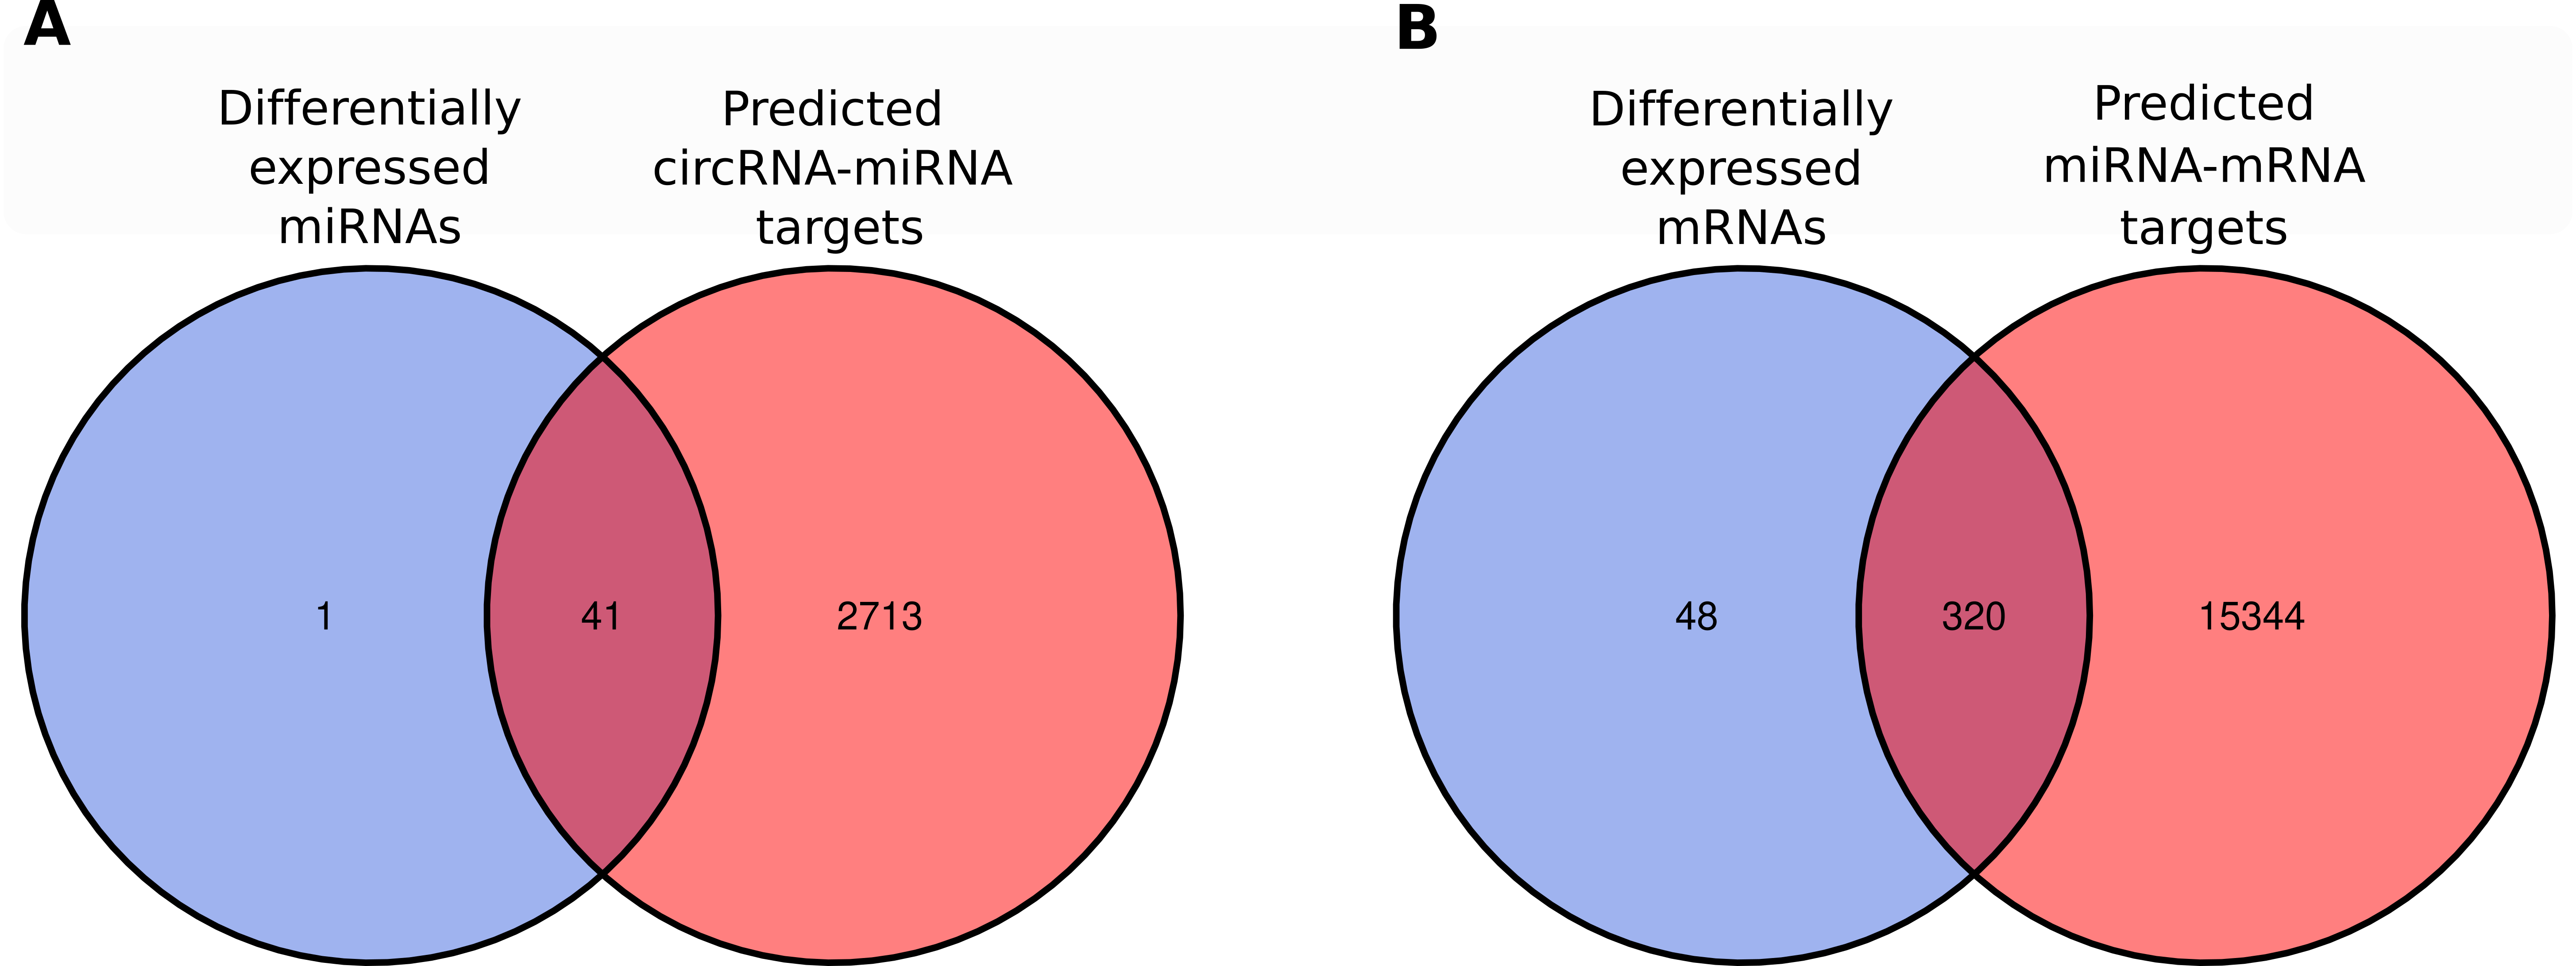
\includegraphics[scale=0.45]{figures/database_overlaps.png}
    \caption{\textbf{(A)} overlap of predicted circRNA-miRNA targets returned by CircBase and CDSC with differentially expressed miRNAs. \textbf{(B)} overlap of predicted miRNA-mRNA targets using Targetscan, miRTarBase, miRNet and miRBase with differentially expressed mRNAs.}
    \label{fig:db_overlaps}
\end{figure*}

\subsection*{\textbf{Construction of ceRNA network}}
Using R, the ceRNA network was subject to a final round of filtering to conform to the hypothesized sponging model between circRNA, miRNAs and mRNAs: 1) the higher the circRNA expression, the lower the miRNA expression and higher the mRNA expression; 2) the lower the circRNA expression, the higher the miRNA expression and lower the mRNA expression. A nodelist and edgelist was exported and visualised using Cytoscape software \cite{Shannon2003Nov} (version 3.10.0 \url{https://cytoscape.org/}).

\begin{figure*}[h!]
  \includegraphics[width=0.97\textwidth]{figures/rearranged_network.png}
  \caption{pathfindR hierarchical clustering of enriched terms. Node sizes correspond to the -log(p-value) for each term, line thickness represents the kappa statistic between terms. The color of each node corresponds to distinct clusters generated by clustering.}
  \label{fig:pathfindRnetwork}
\end{figure*}

\subsection*{\textbf{Enrichment Analysis}}
Active-subnetwork-oriented pathway enrichment analysis was performed on DE-mRNAs in the ceRNA network using pathfindR \cite{Ulgen2019Sep}. KEGG, Reactome and GO gene sets were used to identify active subnetworks (in which interconnected genes predominantly comprise input DE-mRNAs) in the BioGrid protein-protein interaction network (PIN) over 100 iterations. Enriched pathways with a p-value $\leq$0.05 and $\geq$50 occurrences over all iterations were considered significant. Hierarchical clustering was performed on all enriched terms using 1 - kappa statistic as the distance metric to generate a network cluster. The network was rearranged to include clusters with the largest membership in Inkscape vector graphics software.


\subsection*{\textbf{Construction of a prognostic model}}
To assess the prognostic value of the DE-mRNAs returned by the ceRNA network, univariate Cox proportional hazards regression and Benjamini Hochberg multiple testing correction (P$\le$0.05) was conducted using the RegParallel R package \cite{regparallel} on scaled and centred log2 CPM TCGA-PRAD gene expression data to identify biochemical recurrence (BCR) associated genes. Genes that violated the proportional hazard assumptions as determined by scaled Schoenfeld residuals \cite{Schoenfeld1982Apr} were discarded. Next, we constructed a multivariate Cox proportional hazards model using backwards selection via the stepwise Akaike information criterion (stepAIC) MASS function \cite{MASS} with a significance level of P$\le$0.05 to identify the most relevant predictors. \par
A prognostic index (PI) was constructed using the weighted sum of the variables in the model, where the weights are the regression coefficients. The median value of the PI was used to stratify patients into high risk and low-risk strata with the expectation that the high risk group would harbour more biochemical recurrence events and thus have a poorer prognosis than the low-risk group. Kaplan–Meier survival analysis and a log-rank test was employed to formally assess this assumption using the survfit function in the survminer R package \cite{survminer}. Furthermore, the timeROC R package \cite{timeroc} was used to show receiver operating characteristic (ROC) curves, and area under ROC curve (AUC) to evaluate the prediction of the prognostic model for 1, 3, 5 and 8 years biochemical recurrence rates, respectively.

\begin{table*}[ht!]
\caption{4-gene prognostic model obtained from the ceRNA network.}
\begin{tabular}{lllllll}
\toprule
\textbf{Gene} & \textbf{Coef} & \textbf{CI} & \textbf{exp(Coef)} & \textbf{S.E.} & \textbf{Wald Z} & \textbf{P-value}
\\
\toprule
REG4 & -0.392 & (-0.602, -0.181) & 0.676 & 0.107 & -3.65 & 0.00026
\\
SLC2A4 & -0.293 & (-0.509, -0.076) & 0.746 & 0.111 & -2.64 & 0.0082
\\
JAG2 & 0.394 & (0.185, 0.603) & 1.483 & 0.107 & 3.69 & 0.00022
\\
CTHRC1 & 0.419 & (0.196, 0.640) & 1.520 & 0.113 & 3.71 & 0.00021 
\\
\toprule
\end{tabular}
\label{tab:genes_coxph_bcr}
\end{table*}

\begin{figure*}[h!]
    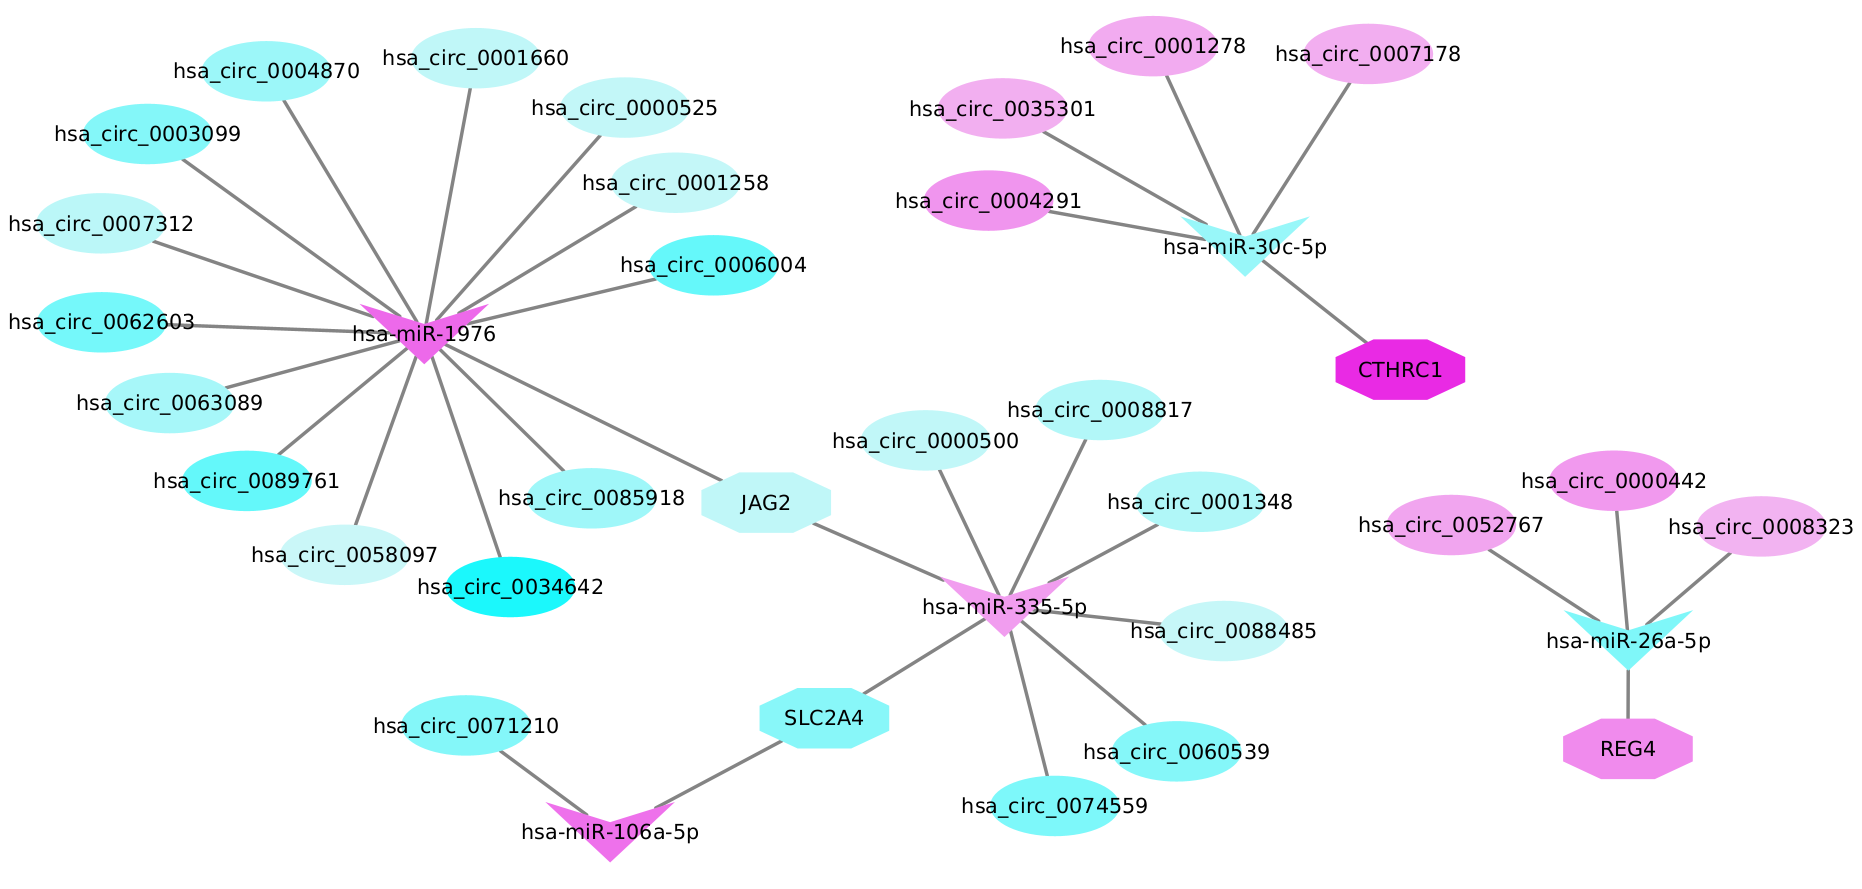
\includegraphics[width=0.96\textwidth]{figures/prognostic_cytoscape.png}
    \caption{The prognostic ceRNA network visualised using Cytoscape. Blue nodes represent down-regulation, pink nodes represent up-regulation in the network. LogFC values were averaged across experiments. Shape key: circRNA (ellipse), miRNA (arrow), mRNA (octagon).}
    \label{fig:cytoscape}
\end{figure*}

\subsection*{\textbf{Construction of a clinical nomogram}}
A univariate and multivariate cox proportional hazards model was constructed to include PI and the clinical covariates age, PSA, Gleason score, pathologic T, pathologic N, clinical M and surgical resection status. To reduce the degrees of freedom in the model, the covariates age, Gleason score and PSA were stratified to produce the categorical variables: age $\geq$ 56/$<$56; Gleason score $\leq$ 6, Gleason score 7 and Gleason score 8, 9 and 10; PSA $<$10ng/ml, PSA 10-20ng/ml and PSA $>$20ng/ml. The optimal cutoff for age was calculated using the maxstat R package \cite{maxstat}. Furthermore, pathologic T was simplified to T2, T3 and T4 status. Next, the transcan function in the Hmisc R package \cite{Hmisc} was used to impute missing values in each covariate before fitting a univariate and multivariate cox regression model. Significant covariates (P$\leq$0.05) with a positive hazard ratio were included in the final nomogram model. The nomogram was constructed using the RMS R package \cite{RMS} and visualized using the regplot R package \cite{regplot}. The prediction accuracy of the overall nomogram and each of its individual predictors was calculated for years 1, 3, 5 and 8 in the TCGA-PRAD dataset via AUC. Furthermore, Harrell's c-index was calculated and compared to the derivation model to assess the clinical models performance. 

\subsection*{\textbf{Model validation on external datasets}}
To validate the 4 gene prognostic model using external datasets, we calculated the discriminative power and overall model fit as suggested in a previous review \cite{Royston2013Dec} in conjunction with ROC analysis to assess model performance: 1) The calibration slope in the validation dataset was computed and compared to the slope of the derivation dataset. A calibration slope $<$1 suggests less discriminative power whilst a slope $>$1 indicates superior discriminative power in the validation dataset. 2) The overall fit of the prognostic model in the validation dataset was computed via a joint test of all predictors whilst constraining the prognostic index to 1. A small Chi-squared test value and non-significant p-value indicate a good fit of the prognostic index in the validation dataset. 3) Harrell's c-index was computed for both the derivation and validation datasets; agreement between the two datasets being indicative of similar predictive performance. 4) Kaplan-Meier survival curves between risk group strata, as defined by the median prognostic index value, were plotted to provide informal evidence of discrimination. 5) Hazard ratios between risk groups were computed in the validation and derivation dataset. Ideally, the hazard ratio in the derivation dataset is well maintained in the validation dataset and remains statistically significant. 6) ROC analysis revealed the overall predictive accuracy of the model via AUC. All external datasets were processed in an identical manner to the derivation dataset as previously described.


\begin{table*}[ht!]
\caption{Evaluation of the derivation dataset and the validation datasets used in the study.}
\begin{tabular}{llllllllll}
\\
 & \multicolumn{3}{c}{\textbf{Calibration slope}} & \multicolumn{2}{c}{\textbf{Chi-squared}} & & \multicolumn{3}{c}{\textbf{High risk stratum}}
\\ \cmidrule(lr){2-4}\cmidrule(lr){5-6}\cmidrule(lr){8-10}
 & \textbf{coef} & \textbf{(95\% CI)} & \textbf{P-value} & \textbf{\(\chi^2_5\)} & \textbf{P-value} & \textbf{Harrell's C} & \textbf{Hazard ratio} & \textbf{(95\% CI)} & \textbf{P-value}
\\
\toprule
TCGA-PRAD & 1.00 & (0.73, 1.26) & $<$0.001 & 0 & 1 & 0.71 & 3.78 & (2.37, 6.03) &	$<$0.001
\\
DKFZ & 1.23 & (0.81, 1.66) & $<$0.001 & 6.03 & 0.644 & 0.79 & 4.79 & (1.78, 12.86) &	0.002
\\
Taylor & 1.04 & (0.20, 1.89) & 0.015 & 5.8 & 0.67 & 0.63 & 2.18 & (0.99, 4.77) &	0.052
\\
GSE54460 & 0.71 & (0.31, 1.11) & $<$0.001 & 6.86 & 0.55 & 0.69 & 3.51 & (1.88, 6.56)	 & $<$0.001
\\
CPC & 0.64 & (0.16, 1.11) & 0.009 & 3.79 & 0.875 & 0.67 & 1.99 & (1.01, 3.89) & 0.045
\\
Stockholm & 0.62 & (0.23, 1.01) & 0.002 & 4.26 & 0.833 & 0.65 & 2.27 & (1.23, 4.16) & 0.008
\\
Belfast & 0.34 & (0.00, 0.68) & 0.051 & 18.27 & 0.019 & 0.61 & 1.81 & (1.06, 3.09) & 0.031
\\
\toprule
\end{tabular}
\label{tab:external_validation}
\end{table*}

\begin{figure*}[ht!]
    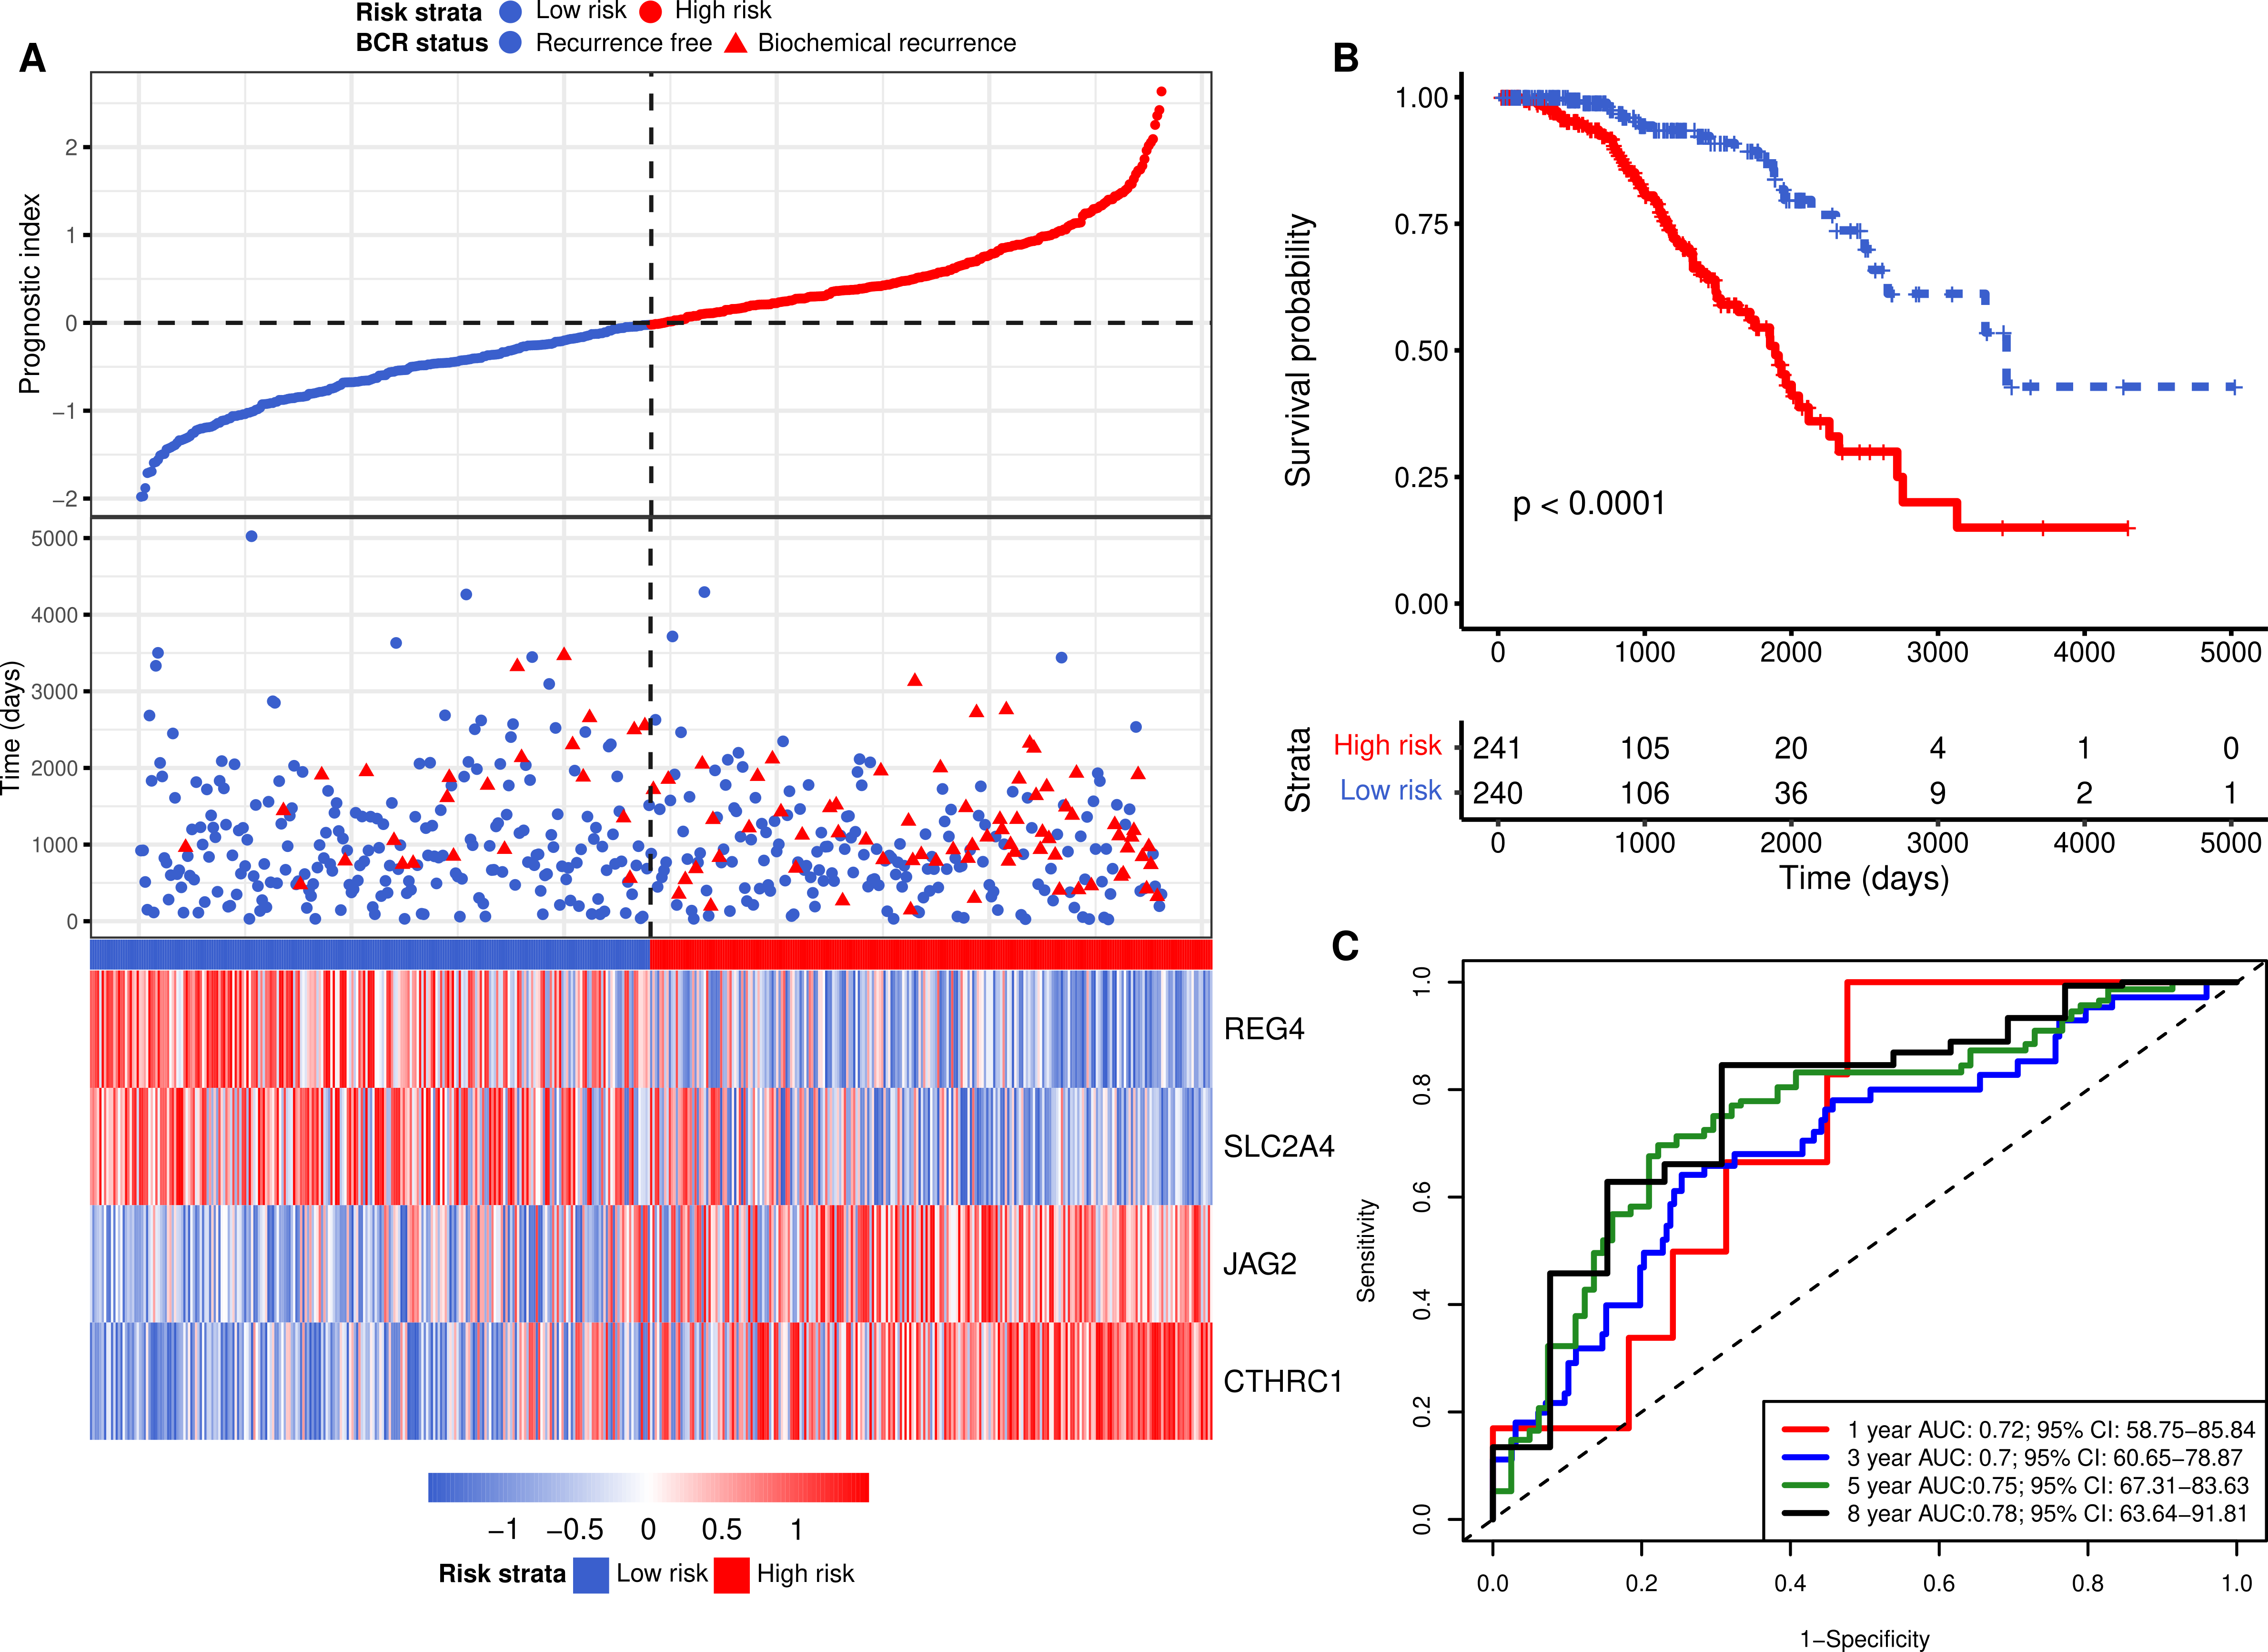
\includegraphics[width=0.95\textwidth]{figures/TCGA_plots.png}
    \caption{The performance of the 4-gene prognostic model in the derivation TCGA-PRAD dataset. \textbf{(A)} The distribution of ranked PI in patients, a scatterplot of BCR status in TCGA-PRAD and a heatmap of the prognostic genes ordered by increasing PI. \textbf{(B)} Kaplan-Meier survival analysis in TCGA-PRAD stratified by high-risk and low-risk groups as defined by the median PI cutoff point. \textbf{(C)} ROC analysis and AUC prediction accuracy of the PI in TCGA-PRAD.}
    \label{fig:tcga_data}
\end{figure*}

\subsection*{\textbf{Estimation of infiltrating cells and tumour purity}}
The Estimation of STromal and Immune cells in MAlignant Tumours using Expression data (ESTIMATE) was obtained for TCGA-PRAD samples via the \href{https://bioinformatics.mdanderson.org/estimate/}{ESTIMATE website} \cite{estimate}. ESTIMATE provides insights into the presence of stroma in tumor tissue, the infiltration of immune cells in tumor tissue and the overall tumor purity via stromal, immune and ESTIMATE scores, respectively. Microenvironment Cell Populations-counter (MCP-counter) was applied to TCGA-PRAD samples to quantify the abundance of CD3\textsuperscript{+} T cells, CD8\textsuperscript{+} T cells, cytotoxic lymphocytes, NK cells, B lymphocytes (B lineage), cells originating from monocytes (monocytic lineage), myeloid dendritic cells, neutrophils, as well as endothelial cells and fibroblasts. Finally, 28 Tumor-Immune System Interaction (TISI) gene sets were downloaded from \href{http://cis.hku.hk/TISIDB/index.php}{TISIDB}. Single-sample GSEA was performed using the GSVA R package \cite{GSVA} to derive per-sample enrichment scores. Student's T-test was performed to delineate differences in immune infiltration and expression in the high-risk and low-risk strata for each of ESTIMATE, MCP-counter and TISIDB scores. 

\begin{figure*}[ht!]
    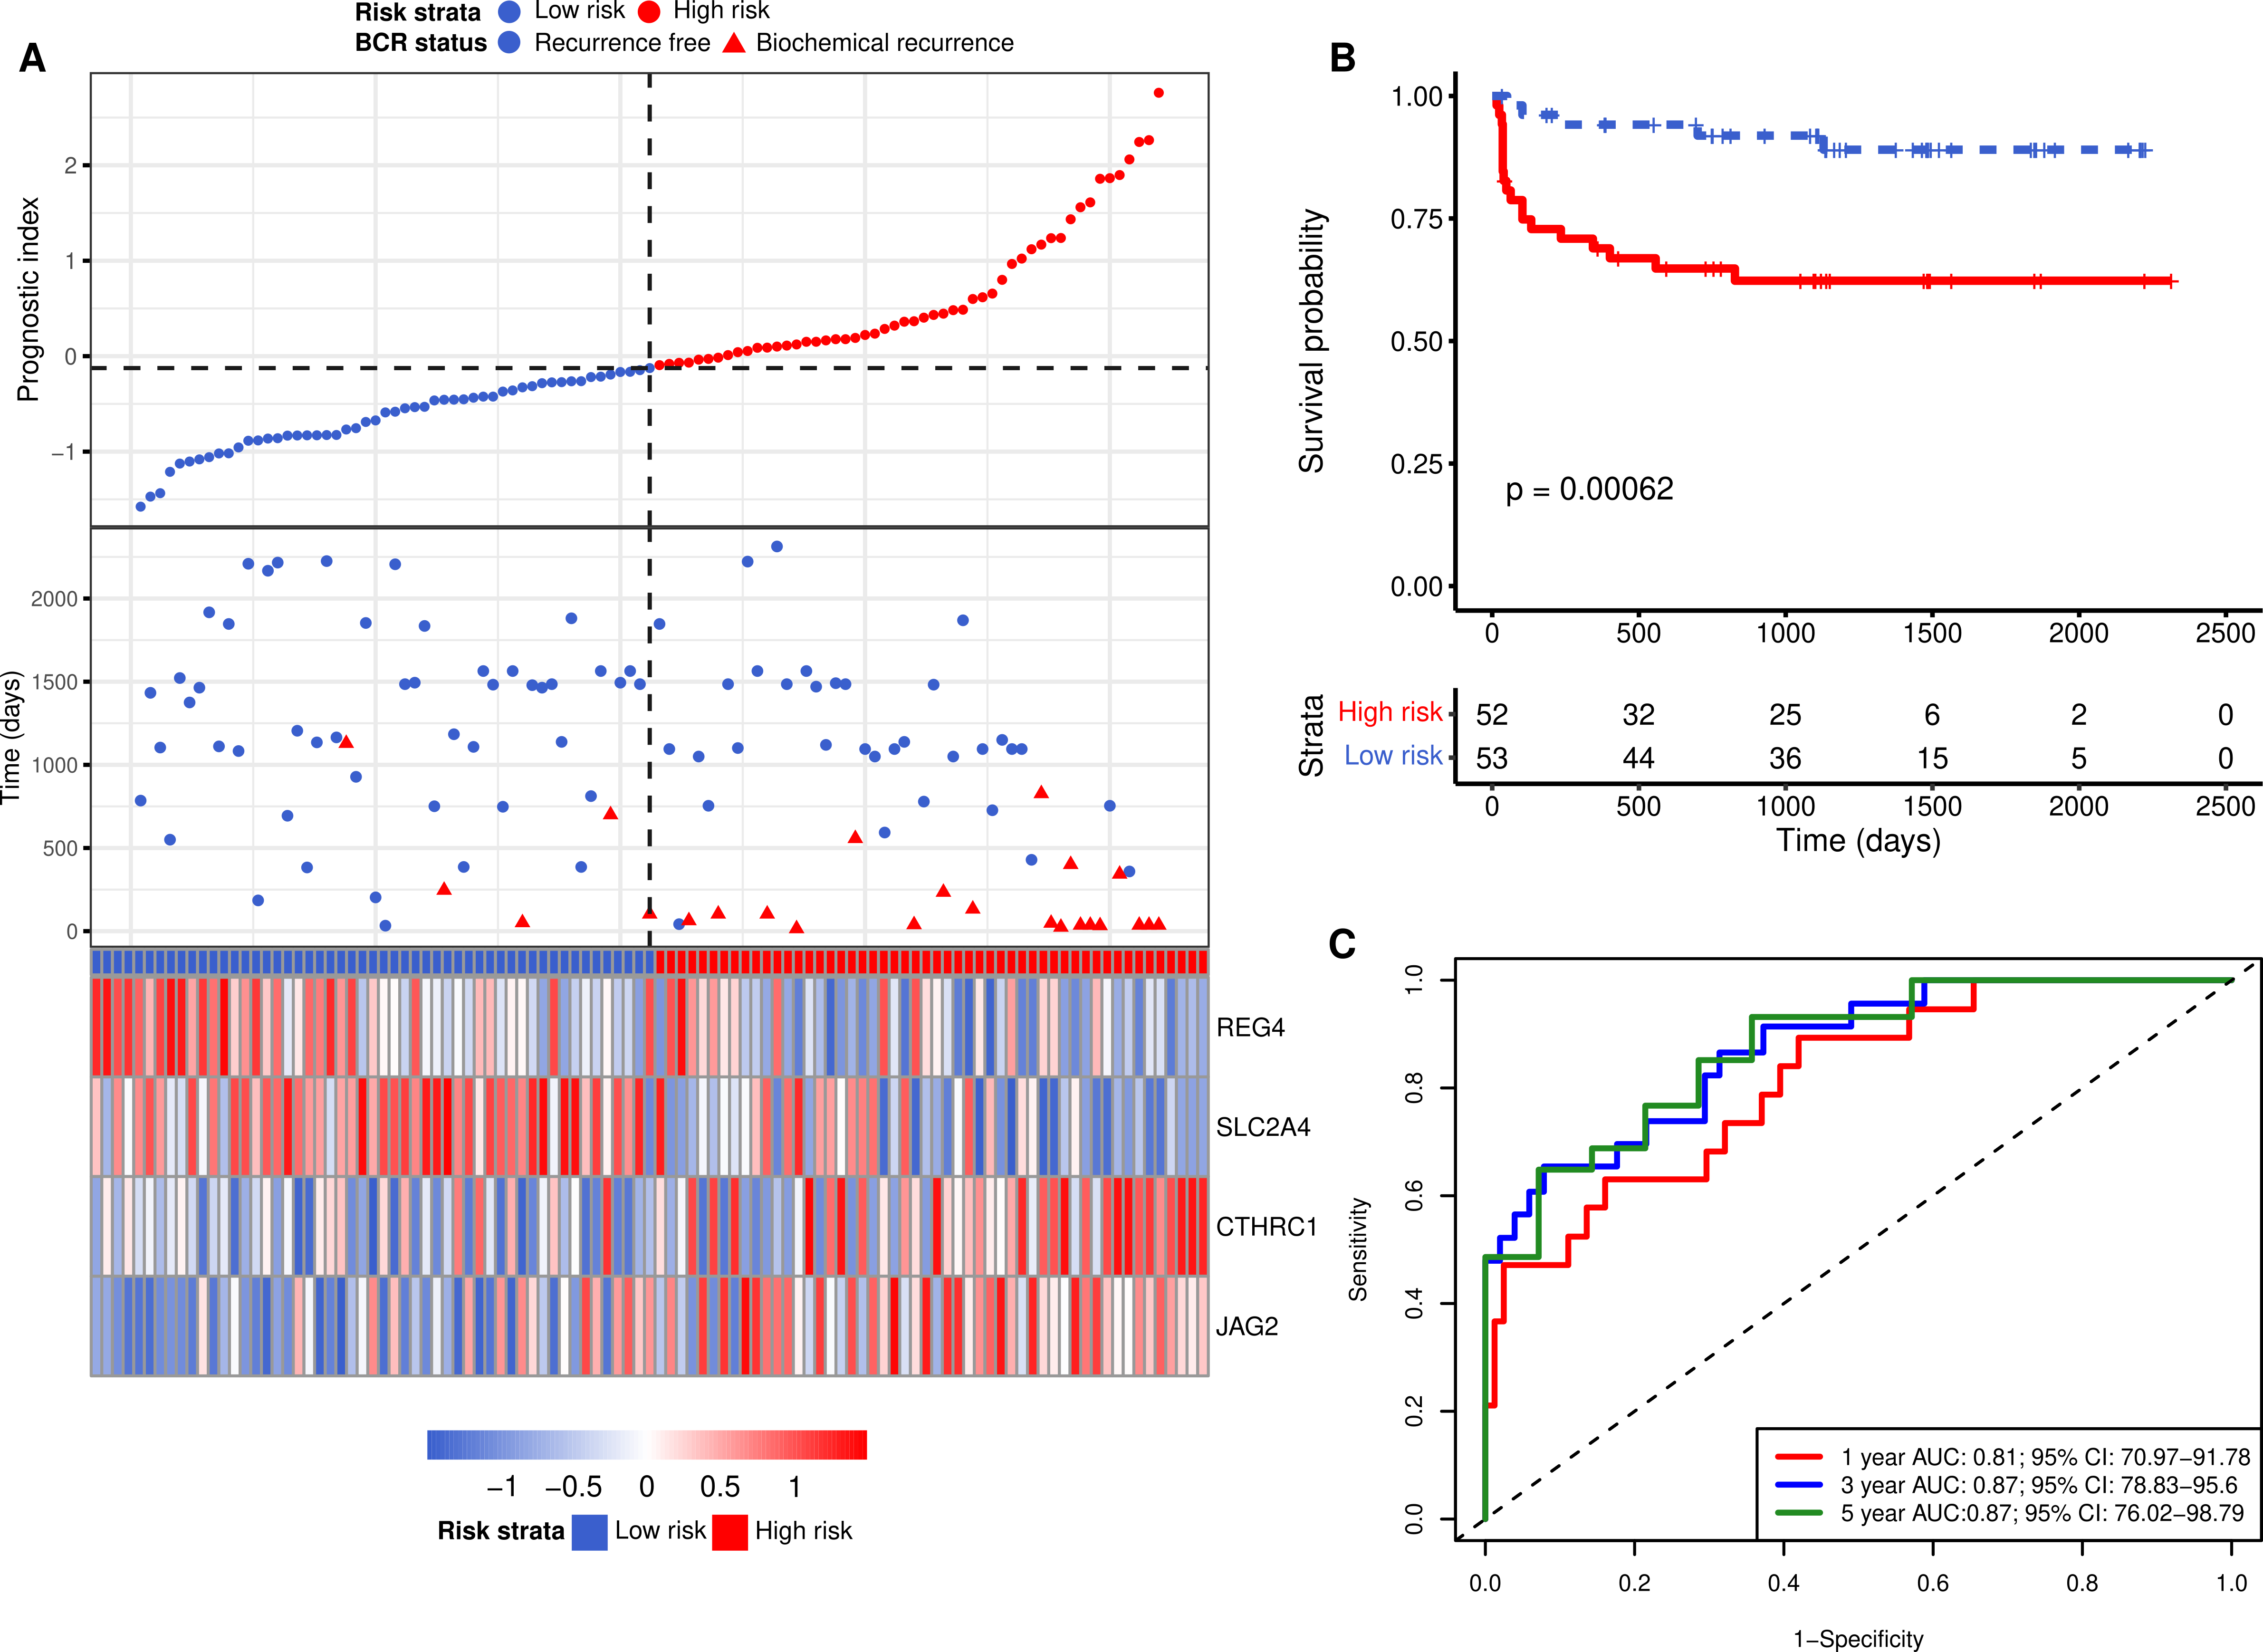
\includegraphics[width=0.95\textwidth]{figures/DKFZ_plot.png}
    \caption{The performance of the 4-gene prognostic model in the validation DKFZ dataset. \textbf{(A)} The distribution of ranked PI in patients, a scatterplot of BCR status in DKFZ and a heatmap of the prognostic genes ordered by increasing PI. \textbf{(B)} Kaplan-Meier survival analysis in DKFZ stratified by high-risk and low-risk groups as defined by the median PI cutoff point. \textbf{(C)} ROC analysis and AUC prediction accuracy of the PI in DKFZ.}
    \label{fig:dkfz_data}
\end{figure*}

\section*{Results}
\subsection*{\textbf{Identification of the ceRNA network}}
Datasets downloaded in the study were subject to differential expression analysis and the downstream intersection of results to derive a common signature in enzalutamide resistance and prostate cancer. The contrasts used in each analysis and the summary of their results are provided in Table \ref{tab:de_results}. Differential circRNA expression analysis revealed 279 DE-circRNAs (174 up-regulated, 105 down-regulated). Target prediction of circRNAs using the CircBase and CDSC databases returned 2754 predicted circRNA-miRNA pairs which were subset using the results of differentially expressed miRNAs (16 up-regulated, 26 down-regulated) to produce a final set of 41 DE-miRNAs (Figure \ref{fig:db_overlaps}A). TargetScan, miRNet, miRTarBase and miRBase returned 15712 miRNA-mRNA target predictions based on the input 41 DE-miRNAs. Predictions were intersected using 368 DE-mRNAs returned by differential gene expression analysis (196 up-regulated, 172 down-regulated), resulting in a set of 320 DE-mRNAs (Figure \ref{fig:db_overlaps}B). The preliminary ceRNA network consisting of 278 circRNAs, 41 miRNAs and 320 mRNAs was subject to filtering based on the ceRNA hypothesis to generate a ceRNA network consisting of 141 circRNAs, 40 miRNAs and 256 mRNAs.
\par
Functional analysis of DE-mRNAs using pathfindR annotated 29, 33 and 57 GO, KEGG and Reactome pathways, respectively (Figure \ref{fig:pathfindRnetwork}). Pathways involved in the epithelial-mesenchymal transition (EMT) were enriched in addition to CASP8 inhibition, protein ubiquitination and SUMOylation pathways contributing to the survival and proliferation of cancer cells within the tumor microenvironment. DARPP-32 and FCERI-mediated Ca2+ mobilization may contribute to the progression of prostate cancer and the acquisition of a chemotherapeutic drug-resistant phenotype.

\begin{figure*}[ht!]
    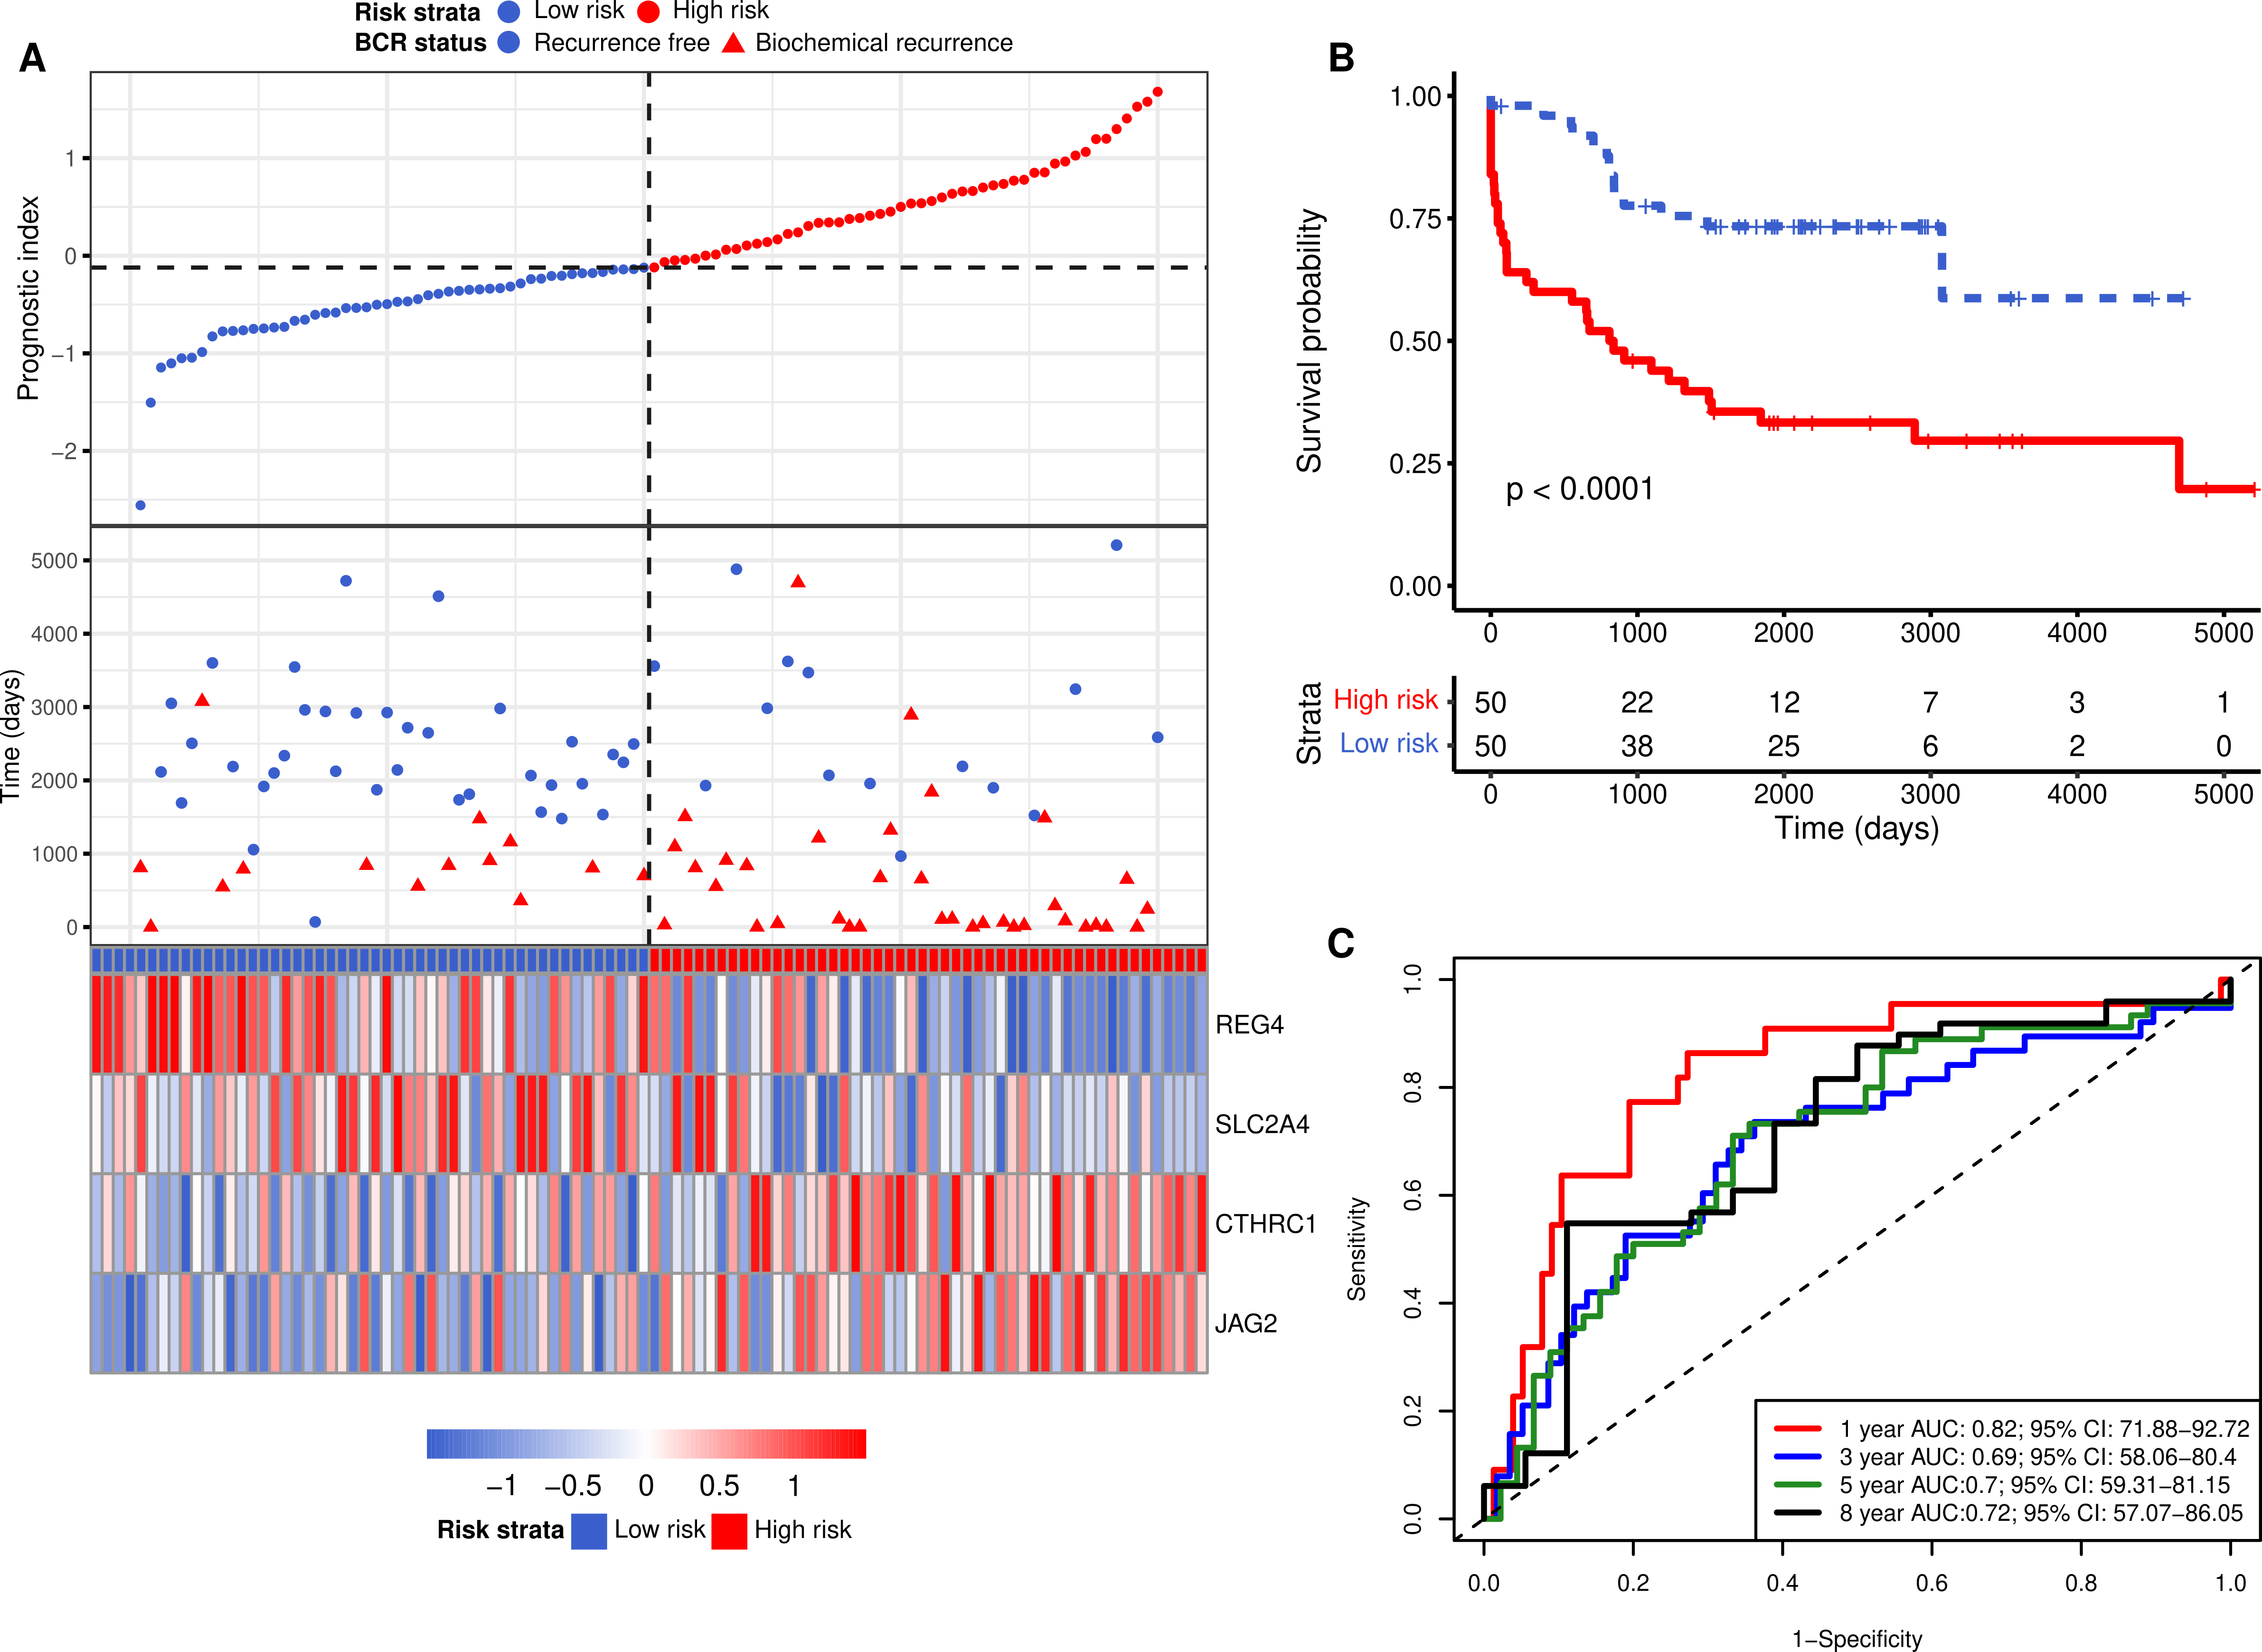
\includegraphics[width=0.95\textwidth]{figures/GSE54660_plot.png}
    \caption{The performance of the 4-gene prognostic model in the validation GSE54660 dataset. \textbf{(A)} The distribution of ranked PI in patients, a scatterplot of BCR status in GSE54660 and a heatmap of the prognostic genes ordered by increasing PI. \textbf{(B)} Kaplan-Meier survival analysis in GSE54660 stratified by high-risk and low-risk groups as defined by the median PI cutoff point. \textbf{(C)} ROC analysis and AUC prediction accuracy of the PI in GSE54660.}
    \label{fig:gse54460_data}
\end{figure*}

\subsection*{\textbf{Prognostic model development}}
The 256 DE-mRNAs returned by the enzalutamide ceRNA network were used to derive a model predictive of BCR in PCa. Univariate Cox regression analysis initially identified 24 genes associated with BCR (Supplementary file \href{https://github.com/BarryDigby/pca_network/blob/main/results/TCGA_DFS/ceRNA_genes_univariate_cox.csv}{1}), of which 4 were discarded for violating the proportional hazard assumptions (Supplementary figure \href{https://github.com/BarryDigby/pca_network/blob/main/results/TCGA_DFS/schoenfeld_residuals.pdf}{1}). A multivariate Cox regression model was fit for the remaining 20 genes and via backward selection, a 7 gene signature was identified (Supplementary file \href{https://github.com/BarryDigby/pca_network/blob/main/results/TCGA_DFS/stepAIC_summary.csv}{2}). After applying a filter of P$\leq$0.05 to the 7 genes, we arrived at a 4 gene signature comprising \textit{REG4, SLC2A4, CTHRC1} and \textit{JAG2}. \textit{REG4} and \textit{SLC2A4} are considered protective against BCR, whilst \textit{CTHRC1} and \textit{JAG2} increase the risk of BRC in PCa patients (Table \ref{tab:genes_coxph_bcr}, Supplementary file \href{https://github.com/BarryDigby/pca_network/blob/main/results/TCGA_DFS/4-gene-gepia.png}{3}). \par

\begin{table*}[ht!]
\caption{Results of univariate and multivariate Cox regression analysis with clinical features.}
\begin{tabular}{lllllll}
\toprule
& \multicolumn{3}{c}{\textbf{Univariate Cox}}  & \multicolumn{3}{c}{\textbf{Multivariate Cox}} \\
    \cmidrule(lr){2-4}\cmidrule(lr){5-7}
\textbf{Variable} & \textbf{Hazard Ratio} & \textbf{(95\% CI)} & \textbf{P-value} & \textbf{Hazard Ratio} & \textbf{(95\% CI)} & \textbf{P-value}
\\
\toprule
\textbf{Age} & & & &
\\
\hspace{1mm} $<$56 & Reference & & &
\\
\hspace{1mm} $\geq$56 & 2.11 & (1.19, 3.73) & \textbf{0.010} & 2.06 & (1.11, 3.81) & \textbf{0.02} 
\\
\textbf{PSA} &  &  &  & 
\\
\hspace{1mm} $<$10ng/ml & (Reference) & & 
\\
\hspace{1mm} 10-20ng/ml & 1.33 & (0.82, 2.15) & 0.248 & 0.99 & (0.60, 1.63) & 0.97
\\
\hspace{1mm} $>$20mg/ml & 1.38 & (0.77, 2.49) & 0.284 & 0.76 & (0.40, 1.44) & 0.40
\\
\textbf{Gleason Score} & & & &
\\
\hspace{1mm} Gleason 6 or lower & Reference & & &
\\
\hspace{1mm} Gleason 7 & 4.46 & (0.60, 32.84) & 0.143 & 3.54 & (0.48,26.34) & 0.22 
\\
\hspace{1mm} Gleason 8,9,10 & 13.78 & (1.91 99.29) & \textbf{0.009} & 4.92 & (0.66, 36.81) & 0.12
\\
\textbf{Pathologic T} & & & &
\\
\hspace{1mm} T2 & Reference & & &
\\
\hspace{1mm} T3 & 4.46 & (2.42, 8.21) & \textbf{$<$0.001} & 2.22 & (1.17, 4.24) & \textbf{0.02}
\\
\hspace{1mm} T4 & 2.45 & (0.55, 11.04) & 0.242 & 0.69 & (0.14, 3.33) & 0.65
\\
\textbf{Pathologic N} & & & & 
\\
\hspace{1mm} N0 & Reference & & & 
\\
\hspace{1mm} N1 & 2.33 & (1.49, 3.64) & \textbf{$<$0.001} & 1.04 & (0.63, 1.73) & 0.87 
\\
\textbf{Clinical M} & & & &
\\
\hspace{1mm} M0 & Reference & & &
\\
\hspace{1mm} M1 & 7.37 & (1.01, 53.80) & \textbf{0.049} & 1.68 & (0.21, 13.57) & 0.63
\\
\textbf{Resection status} & & & & 
\\
\hspace{1mm} R0 & Reference & & & 
\\
\hspace{1mm} R1/R2 & 2.11 & (1.40, 3.19) & \textbf{$<$0.001} & 1.73 & (1.08, 2.79) & \textbf{0.02} 
\\
\hspace{1mm} RX & 1.00 & (0.31, 3.22) & 0.999 & 0.55 & (0.17, 1.84) & 0.33 
\\
\textbf{Prognostic index} & 2.72 & (2.09, 3.54) & \textbf{$<$0.001} & 2.21 & (1.62, 3.01) & \textbf{$<$0.001} 
\\
\toprule
\end{tabular}
\label{tab:clinical_univ}
\end{table*}

\subsection*{\textbf{Evaluation of the prognostic model}}
The prognostic model was firstly evaluated in the derivation TCGA-PRAD dataset by stratifying patients into high-risk and low-risk strata using the median prognostic index, resulting in 241 and 240 patients with 74 and 21 BCR events in each stratum, respectively. Kaplan-Meier survival analysis and a log-rank test revealed high-risk groups are significantly associated with worse BCR prognosis (HR=3.78, CI=(2.37, 6.03), P=$<$0.001) (Table \ref{tab:external_validation}, Figure \ref{fig:tcga_data}B). ROC analysis of the prognostic index as a marker revealed an AUC of 1-year (0.72), 3-years (0.7), 5-years (0.75) and 8-years (0.78) indicating the prognostic index can predict BCR with reasonable accuracy (Figure \ref{fig:tcga_data}C). \par
The model was further evaluated in six external datasets, in some cases outperforming the statistics generated by the derivation dataset (Table \ref{tab:external_validation}) highlighting the robustness of the gene signature in predicting BCR. Of particular note is the performance of the model in the DKFZ and GSE54660 validation datasets. The calibration slope and Harrell's c-index in the DKFZ dataset suggest the model has enhanced classification performance, confirmed by a high AUC of 1-year (0.81), 3-years (0.87) and 5-years (0.87) (Figure \ref{fig:dkfz_data}C). The Hazard ratio generated by the DKFZ dataset for the high-risk stratum (HR=4.79, CI=(1.78, 12.86), P=0.002) and Kaplan-Meier plots coupled with a log-rank test (P=0.00062, Figure \ref{fig:dkfz_data}B) indicate patient stratification using the prognostic index was statistically significant and useful in predicting worse BCR prognosis. The GSE54660 dataset largely preserved the derivation datasets Harrel's c-index and Hazard ratios (C=0.69, HR=3.51, CI=(1.88, 6.56), P=$<$0.001) suggesting the predictive model fit well to the GSE4660 validation dataset (Figure \ref{fig:gse54460_data}B). The predictive accuracy in the GSE54660 dataset was acceptable, with an AUC of 1-year (0.82), 3-years (0.69), 5-years (0.7), and 8-years (0.72) (Figure \ref{fig:gse54460_data}C). In the remaining validation datasets, the prognostic model was indeed useful in creating statistically significant strata via the prognostic index, albeit to a lesser degree as revealed by the logrank test (Taylor P=0.047, CPC P=0.041, Stockholm P=0.0067, Belfast P=0.028, Supplementary figure \href{https://github.com/BarryDigby/pca_network/blob/main/results/external/Belfast/Belfast_plot.png}{2},\href{https://github.com/BarryDigby/pca_network/blob/main/results/external/CPC/CPC_plots.png}{3},\href{https://github.com/BarryDigby/pca_network/blob/main/results/external/Stockholm/Stockholm_plots.png}{4},\href{https://github.com/BarryDigby/pca_network/blob/main/results/external/Taylor/Taylor_plots.png}{5}). Taken together, we demonstrate the utility of the 4-gene prognostic model in predicting BCR in various datasets.


\subsection*{\textbf{Combined clinical nomogram}}
The derivation dataset PI and clinical covariates age, PSA, Gleason score, pathologic T, pathologic N, clinical M and surgical resection status were incorporated in a univariate and multivariate Cox model (Table \ref{tab:clinical_univ}). Encouragingly, the PI was independent of other clinical covariates in the multivariate model (HR=2.21, CI=(1.62, 3.01), P=$<$0.001). The covariates age, pathologic T and resection status remained significant in the multivariate model and were included in the final clinical model. A Harrell's c-index of 0.71 indicated good consistency when including clinical covariates. Furthermore, AUC scores of 1-year (0.76), 3-years (0.76), 5-years (0.78) and 8-years (0.76) (Figure \ref{fig:clinical_data}B) in the clinical model outperformed each of the individual predictors in the clinical model (Figure \ref{fig:clinical_data}D-G) and the prediction accuracy of the derivation model for years 1, 3 and 5 (Figure \ref{fig:dkfz_data}C). Investigating the calibration plot for 8-years in the clinical model reveals the clinical model was over-optimistic in predicting BCR (Figure \ref{fig:clinical_data}C).

\begin{figure*}[h!]
    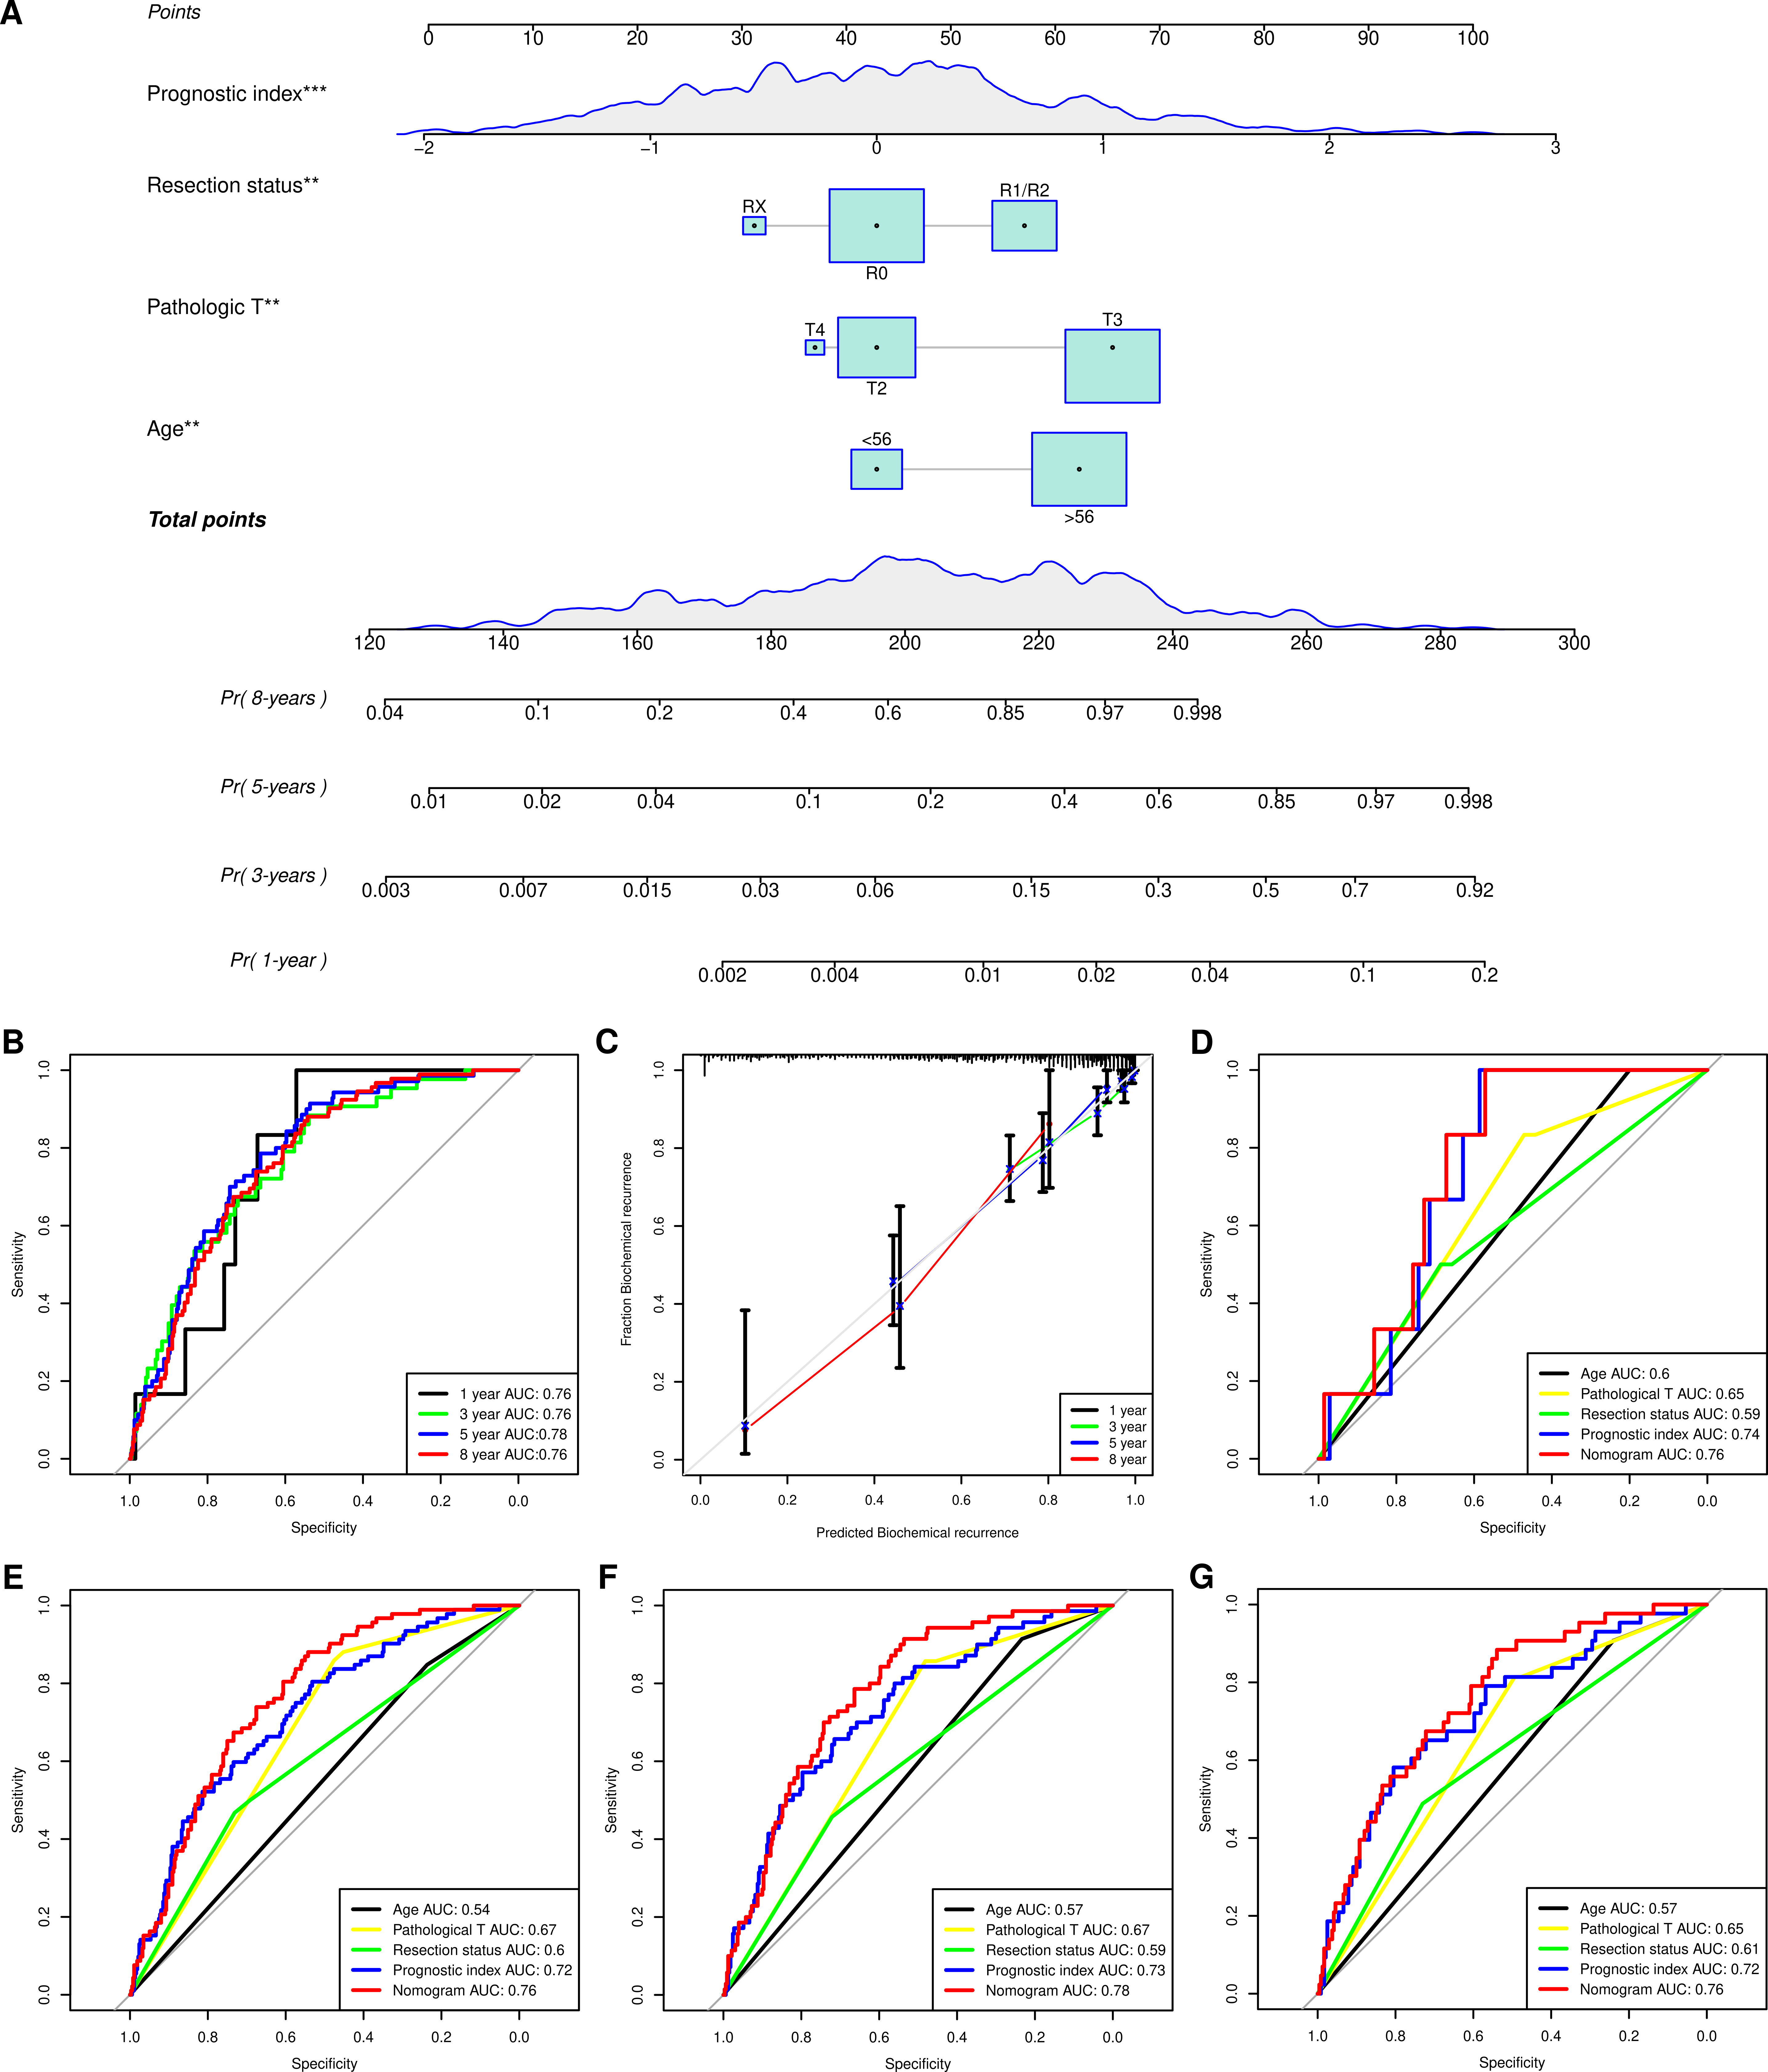
\includegraphics[width=0.95\textwidth]{figures/Clinical_Plots.png}
    \caption{The clinical nomogram and its performance in TCGA-PRAD. \textbf{(A)} Nomogram and its corresponding point scores for each significant predictor. The total points accrued by a patient can be used to predict the probability of a BCR event for years 1, 3, 5 and 8. \textbf{(B)} ROC analysis and AUC predictive accuracy of the nomogram. \textbf{(C)} The calibration of the nomogram, \textit{i.e} its ability to correctly discriminate patients. \textbf{(D-G} ROC analysis and AUC predictive accuracy of the nomogram and each of its individual predictors.}
    \label{fig:clinical_data}
\end{figure*}

\begin{figure*}[h!]
    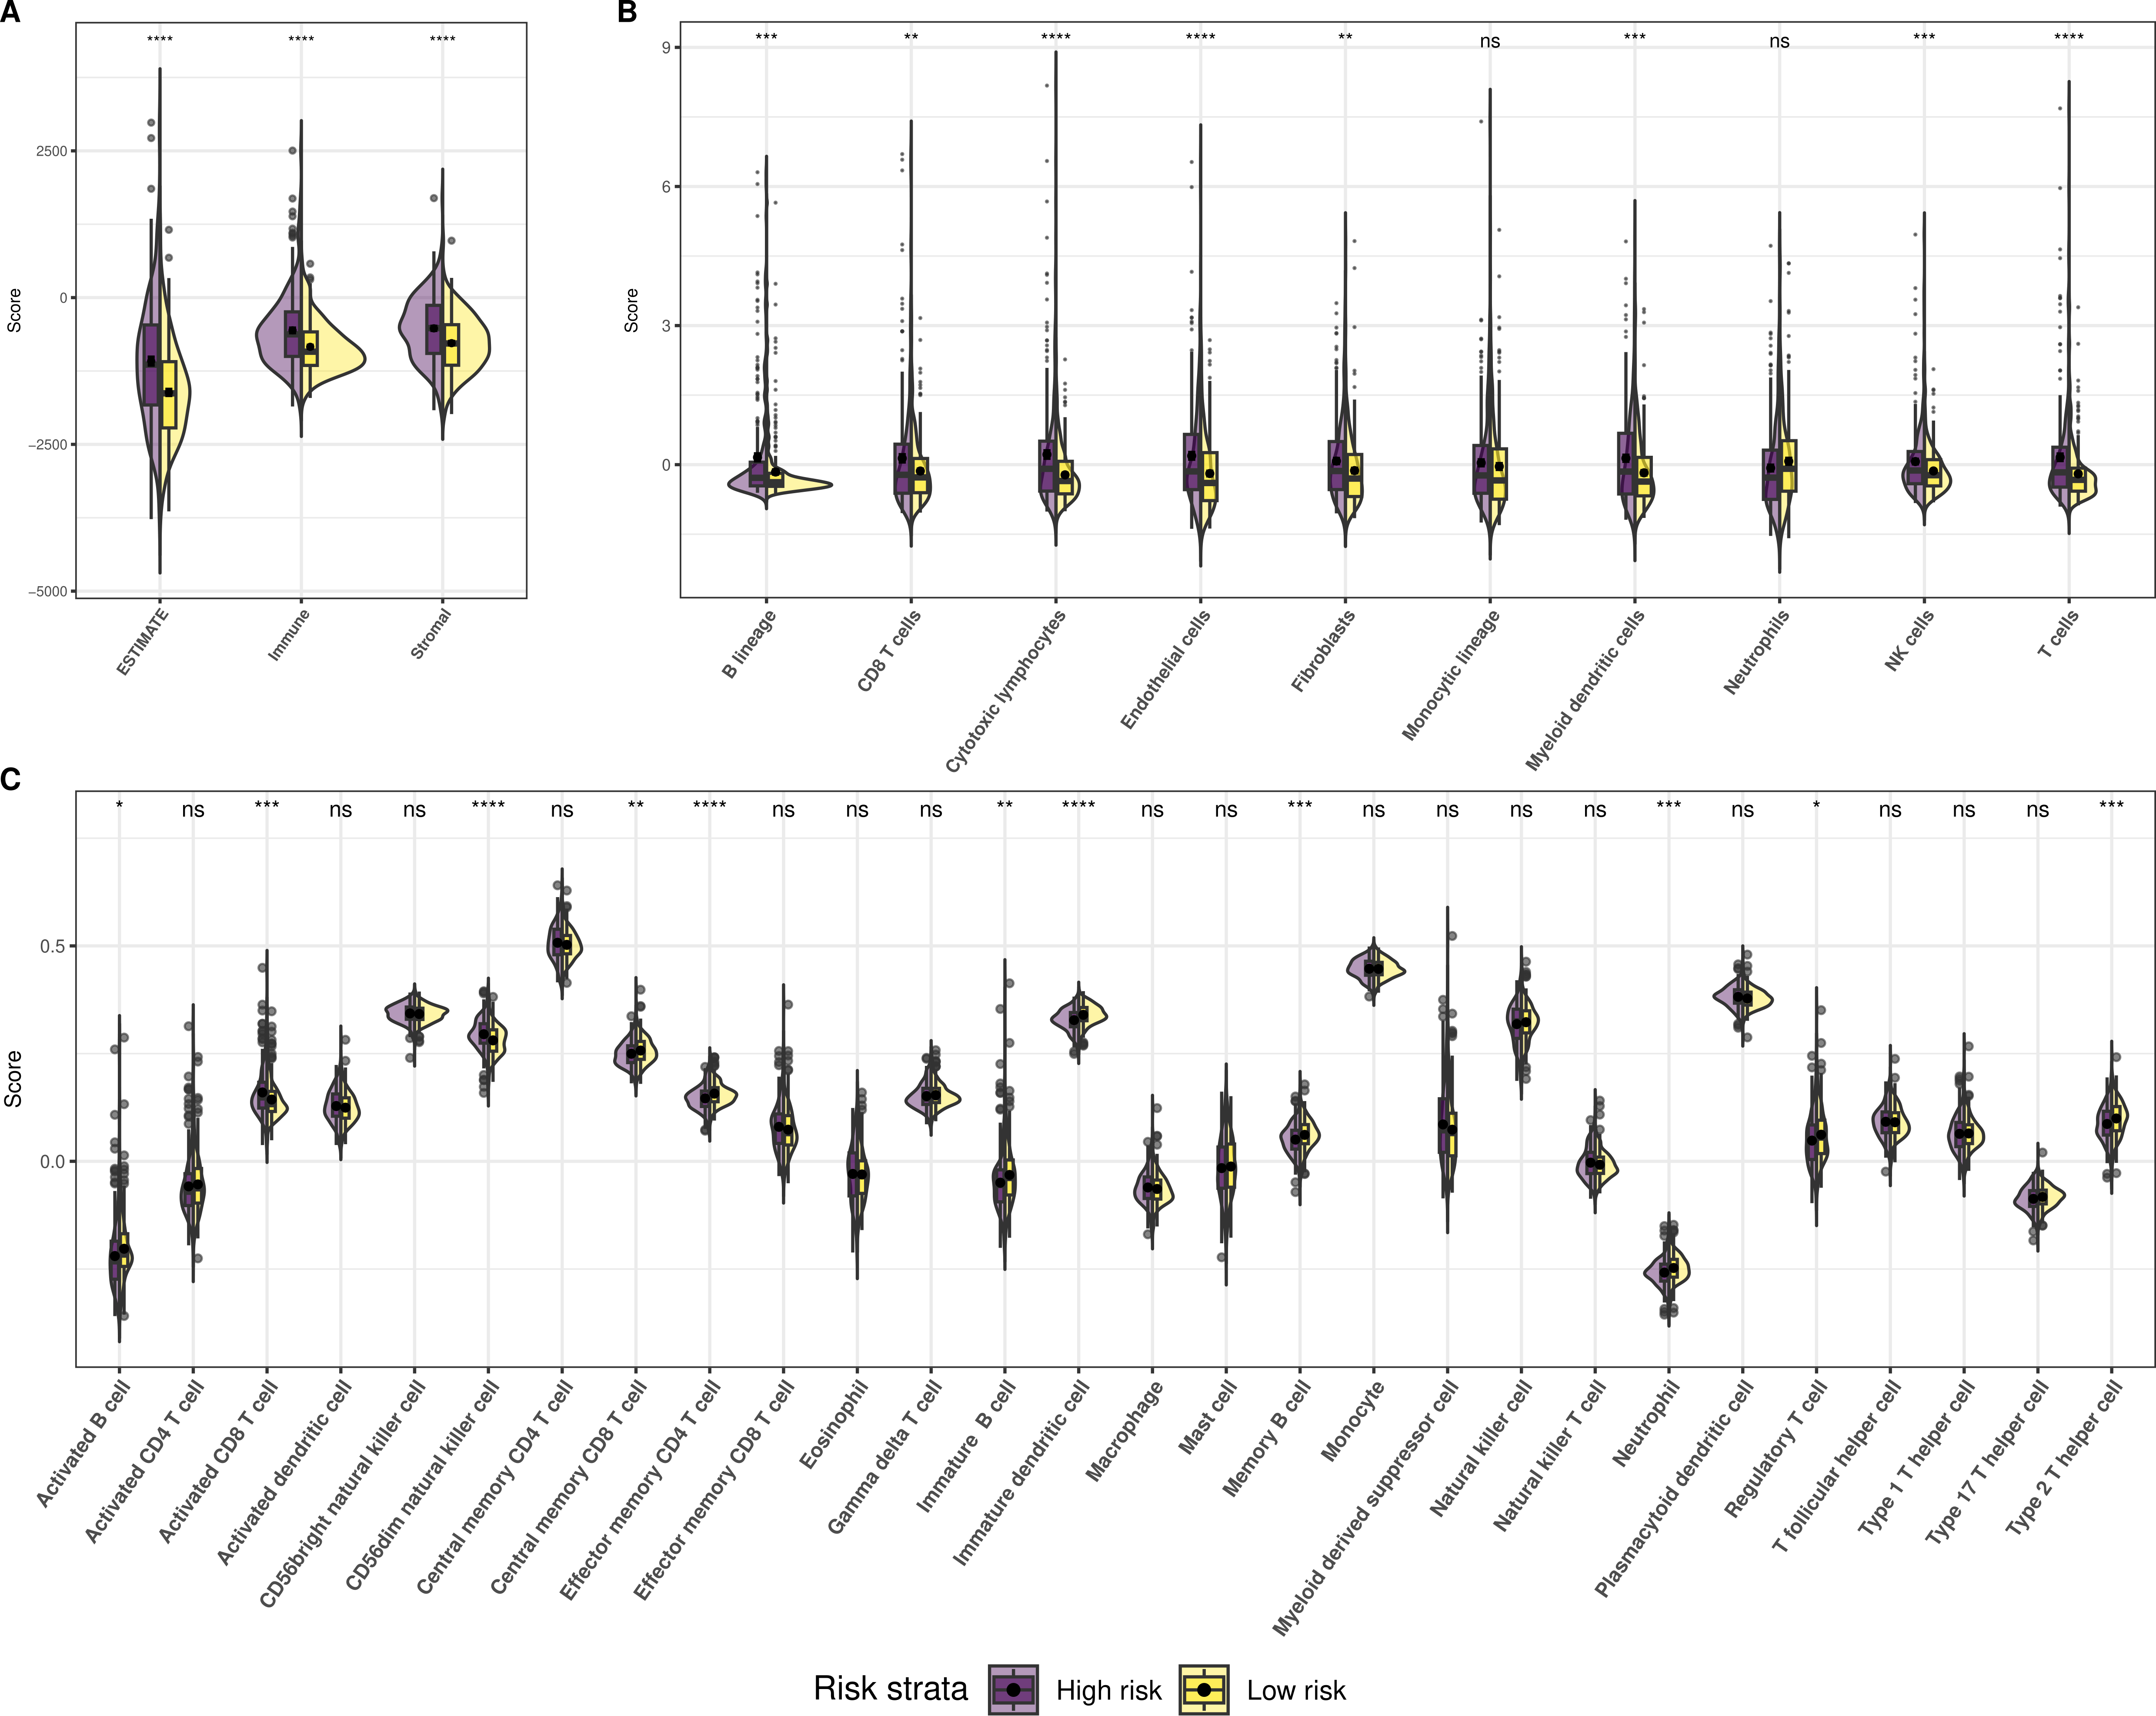
\includegraphics[width=0.95\textwidth]{figures/Immune_plots2.png}
    \caption{Immun infiltration analysis in high-risk and low-risk patient groups. \textbf{(A)} Values returned by ESTIMATE. \textbf{(B)} Enrichment scores returned by MCP-counter. \textbf{(C)} Enrichment scores derived using the 28 immune cell gene sets in TISIDB.}
    \label{fig:immune}
\end{figure*}

\subsection*{\textbf{Immune TME of high-risk and low-risk groups}}
ESTIMATE, MCP-counter and TISIDB immune gene set analysis was performed to elucidate differential immune features in each strata. In the high-risk group, ESTIMATE revealed higher presence of stromal cells, immune cells and tumor purity (P$\leq$0.05, Figure \ref{fig:immune}A). MCP-counter results were all enriched in high-risk patients, except for macrophages and neutrophils which displayed no significant differences between the two strata (Figure \ref{fig:immune}B). Finally, the 28 TISIDB immune gene sets were analysed using ssGSEA. Activated/immature/memory B cells, central/effector memory CD8 T cells, immature dendritic cells, neutrophils, regulatory T cells and type 2 T helper cells were all enriched in low-risk patients. Activated CD8 T cells and CD65dim natural killer cells were enriched in high-risk patients (Figure \ref{fig:immune}C). 

\subsection*{\textbf{Pathways associated with prognostic index}}
To identify functional pathways associated with PI, ssGSEA was performed on KEGG pathways to derive per-patient enrichment scores used as input for subsequent correlation analysis. Pearsons correlation coefficient $>$0.25 and P$\leq$0.05 was deemed significant, resulting in 35 pathways of which 8 were positively correlated with prognostic index, and 27 displayed negative correlation (Figure \ref{fig:kegg_cor}). The majority of pathways related to prognostic index stem from immune responses to pathogen-associated molecular patterns (PAMPs) and damage-associated molecular patterns (DAMPs) suggesting elevated immune activity in high-risk patients. Interestingly, pathways correlated with low-risk patients involved amino acid and fatty acid metbolism hinting at elevated levels of oxidative phosphorylation which when down-regulated, correlates with poor clinical outcomes in several cancer types and the presence of epithelial-to-mesenchymal (EMT) signature \cite{Ahmad2021Oct}.

\begin{figure*}[h!]
    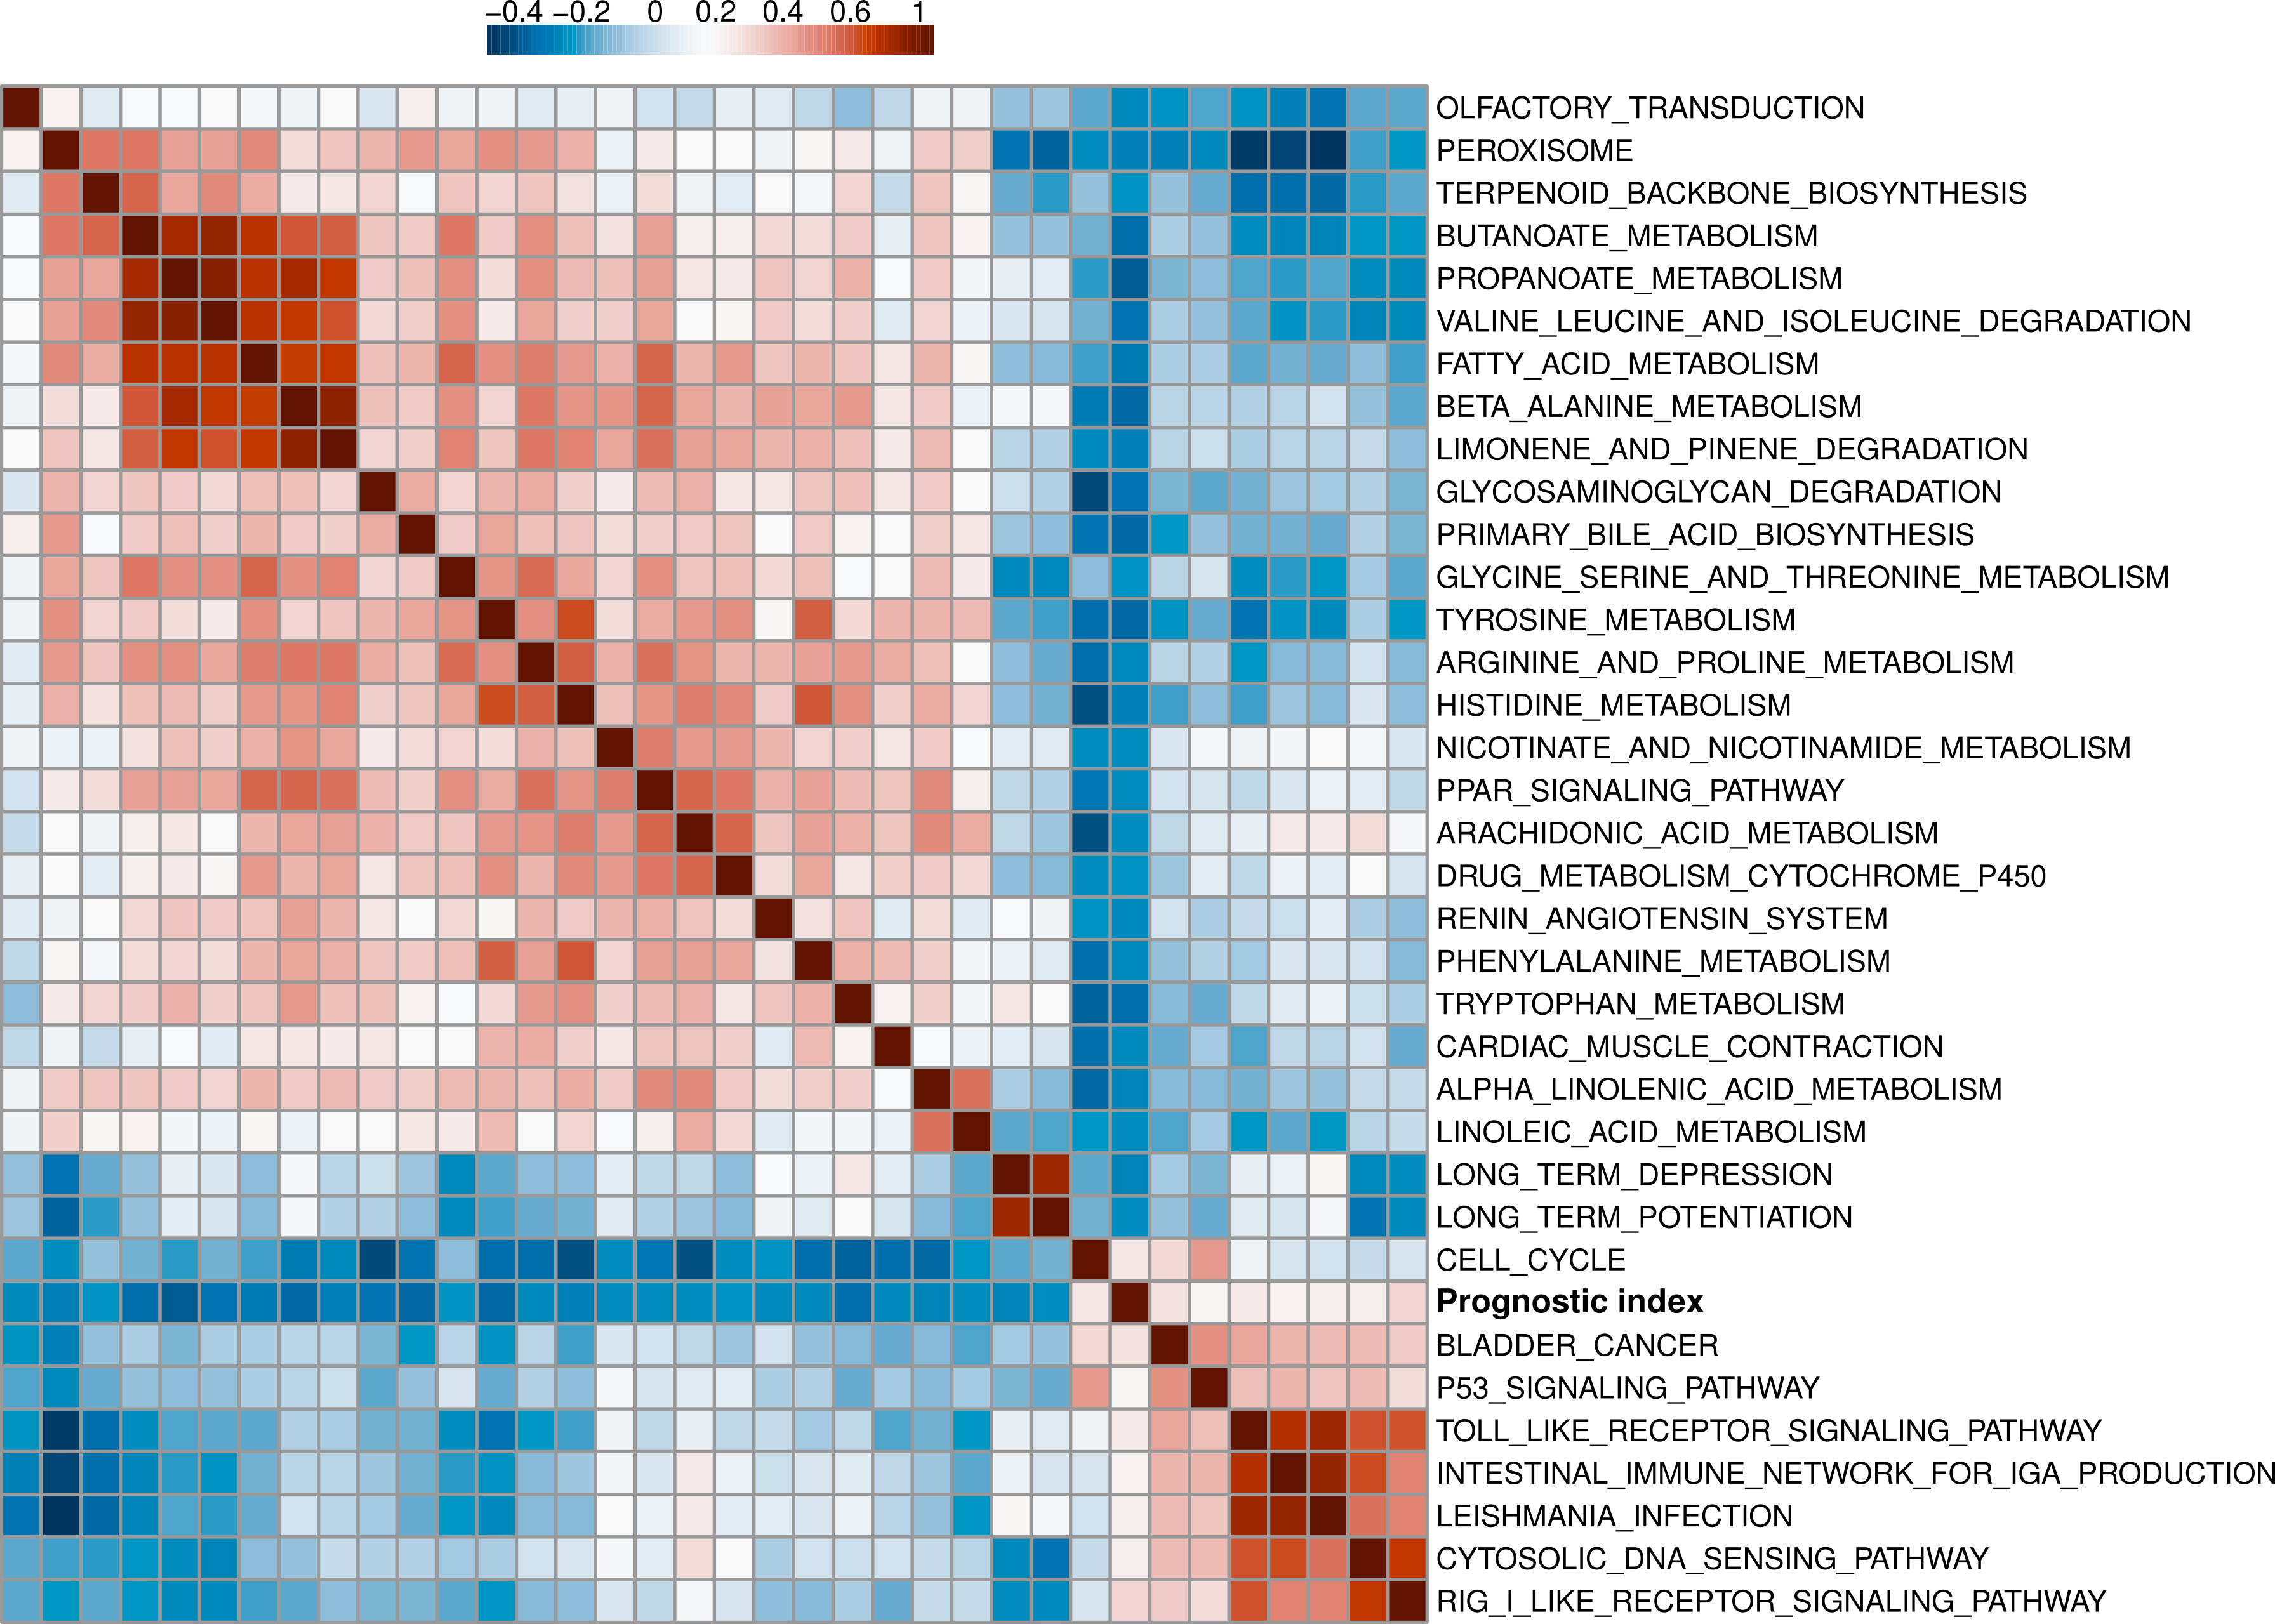
\includegraphics[width=0.95\textwidth]{figures/KEGG_corr.png}
    \caption{Persons correlation of KEGG pathways and the PI returned by the prognostic model.}
    \label{fig:kegg_cor}
\end{figure*}

\section*{Discussion}
We present a 4-gene prognostic signature based on the integration of circRNA-miRNA-mRNA prostate cancer and enzalutamide resistance datasets to gain insights into the mechanism of biochemical recurrence. The 4-gene signature produced a prognostic index from the derivation TCGA-PRAD dataset that effectively stratified patients into high-risk and low-risk strata exhibiting robust performance in the Belfast, CPC, DKFZ, GSE54460, Taylor and Stockholm PCa datasets. Whilst previous studies have generated circRNA-miRNA-mRNA regulatory networks in prostate cancer \cite{Luo2021Dec}, to the best of our knowledge, this work represents the first study that provides a prognostic signature and corresponding prognostic index for use in external validation datasets. We also demonstrate the independence of the prognostic index in relation to clinical features, deriving a clinical nomogram that outperforms the performance of the prognostic index in standalone use. Finally, we elucidate the differential immune features in high-risk and low-risk groups via immune infiltration analysis to identify potential immune biomarkers in prostate cancer. \par
Through literature searches, we further assessed the prognostic ceRNA network (Figure \ref{fig:cytoscape}). hsa-circ-0000442, expressed by the \textit{MED13L} gene, has been demonstrated to exert a tumor-suppressing role in breast cancer \cite{Zhang2021Jan}. In our analysis, we observed up-regulation of hsa-circ-0000442 which is predicted to sequester hsa-miR-26a-5p thereby preventing the post-transcriptional degradation of \textit{REG4}. Our prognostic signature indicates \textit{REG4} is protective against biochemical recurrence hence up-regulation of the hsa-circ-0000442 circular transcript may be linked with improved disease-free survival. hsa-circ-0001258 (parent gene \textit{PPP6R2}) was found to be down-regulated in osteosarcoma chemoresistance groups compared to chemosensitive groups. Transfection of osteosarcoma cells with hsa-circ-0001258 expression vector revealed suppressed doxorubicin resistance \cite{Zhu2019Mar}. In our study we report similar fold change direction of hsa-circ-0001258 in enzalutamide-resistant cells, hinting that the circRNA may play a role in drug resistance. The miRNA hsa-miR-106a-5p is highly expressed in prostate cancer cells vs normal and high grade (Gleason $>$7) tumors vs low-grade tumours and is associated with poor disease-free survival \cite{Hoey2018Aug}. Despite our study demonstrating similar expression levels for hsa-miR-106a-5p, it's predicted role in degrading \textit{SLC2A4} transcripts was shown to be a protective factor against biochemical recurrence. Our study also demonstrated the down-regulation of hsa-miR-26a-5p, confirmed to be significantly decreased in prostate cancer tissues compared with controls in prostate cancer cell lines VCaP, 22RV1, LNCaP, and DU-145 \cite{Guo2016Sep}. \par
\textit{JAG2} (Jagged Canonical Notch Ligand 2) is a member of NOTCH ligands involved in the NOTCH signalling pathway. \textit{JAG2} has been implicated with tumor progression in bladder cancer \cite{Chen2020Jul}, lung cancer \cite{Yang2011Apr} and colorectal cancer \cite{Vaish2017Aug} however, due to the pleiotropic nature of \textit{JAG2} in cells, its value as a prognostic marker is largely cancer-specific. Whilst prostate cancer patients with Gleason scores $\geq$8 exhibited up-regulation of \textit{JAG2} \cite{Ross2011Oct}, our results contradict these findings; \textit{JAG2} was down-regulated in TCGA-PRAD and enzalutamide-resistant cells. \textit{CTHRC1} (Collagen Triple Helix Repeat Containing 1) knockdown suppressed prostate cancer cell proliferation, migration and invasion. The authors also demonstrated that \textit{CTHRC1} was negatively regulated by miR-30e-5p \cite{Ma2020Apr}. In our study, we show that up-regulation of hsa-circ-0004291, hsa-circ-0035301, hsa-circ-0001278, hsa-circ-0007178 potentially inhibits miR-30c-5p, resulting in up-regulation of \textit{CTHRC1}. The interplay between the miR-30 family and \textit{CTHRC1} therefore warrants further investigation. Studies of \textit{REG4} (Regenerating Family Member 4) generally agree with our findings: utility as an independent prognostic marker of relapse after radical prostatectomy \cite{Ohara2008Aug} and similarly elevated expression in tumour prostate cancer cells vs. normal \cite{Gu2005Mar}. Our study found that \textit{SLC2A4} (Solute Carrier Family 2 (Facilitated Glucose Transporter), Member 4 - commonly denoted as \textit{GLUT4}) was downregulated in prostate cancer and enzalutamide resistance, exhibiting a protective effect against BCR. Of note, \textit{SLC2A4} was downregulated in high-risk patients compared to low-risk. Metformin has been shown to induce \textit{SLC2A4} translocation to the cell surface \cite{Lee2012Dec}, enhancing the effects of the antiandrogen bicalutamide and enzalutamide in CRPC patients \cite{Spratt2013Apr,Colquhoun2012Dec,Liu2017Aug}. We therefore propose downregulation of \textit{SLC2A4} may serve as a prognostic marker in prostate cancer patients. 

\section*{Conclusions}
To conclude, this study leveraged existing and novel circRNA-miRNA-mRNA datasets to derive a prognostic signature with robust performance in multiple datasets. It represents the first work deriving a prognostic gene signature based on the competing endogenous RNA network hypothesis involving circRNAs. In addition to the prognostic value of the signature, the 4 genes emerged as candidates for further understanding the mechanism of biochemical recurrence in prostate cancer. 


%%%%%%%%%%%%%%%%%%%%%%%%%%%%%%%%%%%%%%%%%%%%%%
%%                                          %%
%% Backmatter begins here                   %%
%%                                          %%
%%%%%%%%%%%%%%%%%%%%%%%%%%%%%%%%%%%%%%%%%%%%%%

\begin{backmatter}

\section*{Additional Files}
Pilib - hyperlinks to the documents are temporary placeholders. 

\section*{Abbreviations}%% if any
To do 

\section*{Acknowledgements}%% if any
We thank Dr. Marvin Lim and Dr. Elaine Kenny for the preparation and sequencing of the in-house LNCaP cell lines.

\section*{Authors' contributions}
B.D. designed and performed the analysis and drafted the manuscript. P.\`{O}.B. and S.P.F. supervised the work, gave feedback, and revised the manuscript.

\section*{Availability of data and materials}%% if any
The code used to perform the analysis is freely available at \href{https://github.com/BarryDigby/pca_network}{https://github.com/BarryDigby/pca\_network}. Due to file size constraints, files $\geq$20MB used in the analysis are unavailable. The authors can provide these files upon reasonable request.

\section*{Funding}%% if any
Open access and PhD scholarship funding for B.D. provided by Science Foundation Ireland, grant number 18/CRT/6214. No funding body played any role in the design of the study and collection, analysis, interpretation of data or in writing the manuscript.

\section*{Competing interests}
The authors declare that they have no competing interests.

\section*{Ethics approval and consent to participate}%% if any
Not applicable. 


%%%%%%%%%%%%%%%%%%%%%%%%%%%%%%%%%%%%%%%%%%%%%%%%%%%%%%%%%%%%%
%%                  The Bibliography                       %%
%%                                                         %%
%%  Bmc_mathpys.bst  will be used to                       %%
%%  create a .BBL file for submission.                     %%
%%  After submission of the .TEX file,                     %%
%%  you will be prompted to submit your .BBL file.         %%
%%                                                         %%
%%                                                         %%
%%  Note that the displayed Bibliography will not          %%
%%  necessarily be rendered by Latex exactly as specified  %%
%%  in the online Instructions for Authors.                %%
%%                                                         %%
%%%%%%%%%%%%%%%%%%%%%%%%%%%%%%%%%%%%%%%%%%%%%%%%%%%%%%%%%%%%%

% if your bibliography is in bibtex format, use those commands:
\bibliographystyle{bmc-mathphys} % Style BST file (bmc-mathphys, vancouver, spbasic).
\bibliography{bmc_article}      % Bibliography file (usually '*.bib' )
% for author-year bibliography (bmc-mathphys or spbasic)
% a) write to bib file (bmc-mathphys only)
% @settings{label, options="nameyear"}
% b) uncomment next line
%\nocite{label}

% or include bibliography directly:
% \begin{thebibliography}
% \bibitem{b1}
% \end{thebibliography}

\end{backmatter}
\end{document}
